\documentclass[11pt,a4paper,onecolumn]{report}
\usepackage{amsmath}
\usepackage{mathtools}
\usepackage{lmodern}
\DeclarePairedDelimiter{\abs}{\lvert}{\rvert}
\usepackage{bm}
\usepackage[margin=2cm]{geometry}
\usepackage{array}
\usepackage{physics}
\usepackage{amssymb}
\usepackage{textcomp}
\usepackage[T1]{fontenc}
\usepackage{gensymb}
\usepackage{graphicx}
\usepackage{fancyhdr}
\usepackage{enumerate}
\pagestyle{fancy}
\setlength{\headheight}{13.6pt}

\usepackage{tikz}
\usetikzlibrary{shapes.geometric, arrows, calc}
\usepackage[nottoc, numbib]{tocbibind}
\tikzstyle{cool} = [rectangle, rounded corners, minimum width=3cm, minimum
height=1cm, text centered, draw=black, fill=gray!30, text width=3cm]
\tikzstyle{arrow} = [thick, ->, >=stealth] \tikzstyle{line} = [thick, -,
>=stealth]

\usepackage[detect-all]{siunitx}
\usepackage{dsfont}
\usepackage{breqn}
\usepackage{subfigure}
\usepackage{geometry}
\usepackage{listings}
\usepackage{caption}
\usepackage[utf8]{inputenc}
\usepackage{hyperref}
\usepackage{titlesec}
\usepackage[square,numbers,comma,compress]{natbib}
\usepackage{upgreek}
\usepackage{aas_macros}
\usepackage{doi}
\usepackage{siunitx}
\usepackage{textgreek}


\geometry{a4paper, left=25mm, top=25mm,} % total={160mm,247mm} <- overspecification
\graphicspath{{figures/} }
\renewcommand{\listfigurename}{Figures}


\captionsetup{justification   = raggedright, singlelinecheck = false}

\hypersetup{colorlinks, citecolor=black, filecolor=black, linkcolor=black,
    urlcolor=black}

\renewcommand{\bibname}{References}

\bibpunct{(}{)}{;}{a}{}{,}

\hypersetup{colorlinks, citecolor=black, filecolor=black, linkcolor=black,
    urlcolor=black}

% table of contents:
\setcounter{tocdepth}{1}

\newcommand*\chem[1]{\ensuremath{\mathrm{#1}}}

\newcommand{\threevdots}{%
  \vbox{\baselineskip1ex\lineskiplimit0pt%
  \hbox{.}\hbox{.}\hbox{.}}}



% diagnose: Label(s) may have changed. Rerun to get cross-references right.
% \def\@testdef #1#2#3{% \def\reserved@a{#3}\expandafter \ifx \csname
% #1@#2\endcsname \reserved@a  \else \typeout{^^Jlabel #2 changed:^^J%
% \meaning\reserved@a^^J% \expandafter\meaning\csname #1@#2\endcsname^^J}%
% \@tempswatrue \fi}


%opening
% \title{Predicting the Magnetic Field of the Solar Farside}
% \author{Cameron Smith\\
% Student ID: 28792912\\
% Supervisors: Andrew Casey, Alina Donea}
% \date{\today}



\begin{document}


\begin{titlepage}
  \begin{center}
    \vspace*{2cm}
    \Huge
    \textbf{Predicting the Magnetic Field of the Solar Farside}

    \vspace{2cm}
    \LARGE
    \textbf{Cameron Smith}

    \vspace{0.8cm}
    \Large \textit{Supervisors:}\\
    Andrew Casey\\
    Alina Donea

    \vfill
    \large
    An honours thesis presented for the degree of\\
    Bachelor of Science Advanced - Research (Honours)

    \vspace{0.3cm}
    \includegraphics[width=0.2\linewidth]{"Monash_Logo"}\\
    School of Physics and Astronomy\\
    Faculty of Science\\
    Monash University\\
    Australia

    \vspace{0.5cm}

    \today

  \end{center}
\end{titlepage}

\chapter*{Abstract}
Active regions on the Sun's surface can lead to large eruptions with the
potential to cause significant hazards on Earth. Images of the magnetic field on
the Sun's surface, known as magnetograms, are a vital tool for predicting these
events. While these are readily available for the near hemisphere of the Sun,
there is currently no reliable way to generate magnetograms for the far
hemisphere. Consequently, dangerous farside active regions may rotate towards
Earth with little warning. Here we describe a method to generate synthetic
farside magnetograms using a deep learning method applied to helioseismology
data. While the synthetic magnetograms fail to accurately determine the position
or shape of active regions, they successfully predict sharp changes in the total
unsigned magnetic field - a key predictor of solar eruptions.

% \chapter*{Acknowledgements}
%TODO:

% Andy and Alina for their support and invaluable feedback
% Bernhard being very accomadating and willing to help/spend time and effort to
% ensure we weren't adversaly effected by lockdowns/etc

% Friends and family and lovely girlfriend for keeping me sane, and making my
% offtime so much more enjoyable

% Everyone mentioned a huge contribution into making the past year and
% especially the past semester much more pleasant


\tableofcontents


% \listoffigures







%
%
%
%
\chapter{Introduction}
%
%
%
%

A self-regenerating dynamo within the Sun produces a rich and complex solar
magnetic field. Perhaps the most obvious manifestations of this magnetic field
are active regions, which are produced by rising toroidal magnetic flux ropes
that penetrate the solar surface. These active regions are home to extreme
magnetic fields with strengths typically exceeding 1000 Gauss. If an active
region cannot effectively dissipate the electric currents that flow within, a build-up
of magnetic energy can lead to an explosive magnetic reconnection event. These
reconnection events can result in solar flares or coronal mass ejections that
can be dangerous when directed towards Earth. Such events, and associated
geomagnetic storms, have been known to result in an array of technological
disruptions, including blackouts \citep{odenwald_day_2015}, loss of satellites
\citep{carlowicz_did_1997}, and even the detonation of sea mines
\citep{knipp_little-known_2018}. Furthermore, these events have the potential to
cause radiation exposure to astronauts \citep{hu_modeling_2009} and could cause
significant damage to terrestrial electrical grids
\citep{council_severe_2008}. \\


Solar magnetograms, images of the magnetic field of the Sun, are a vital tool
for predicting such events and identifying high-risk active regions before they
erupt
\citep{song_statistical_2009,yuan_solar_2010,lan_automated_2012,bobra_solar_2015,
chen_identifying_2019}. However, solar magnetograms are only available for the
`nearside': the hemisphere of the Sun that faces the Earth. Due to the rotation
of the Sun, active regions that emerge on the `farside' could be facing the
Earth only seven days after becoming visible. A method for producing farside
magnetograms is therefore necessary to provide warning of dangerous farside
magnetic activity before it reaches the Earth. \\


NASA's Solar Terrestrial Relations Observatory (STEREO) has provided some
monitoring of the solar farside throughout its mission. However, STEREO is not
capable of producing magnetograms and only has a partial view of the solar
farside, a view that will only decrease until it passes the Earth in 2023.
Furthermore, one of the two spacecraft comprising the STEREO mission (STEREO-B)
has already lost contact with Earth, while the other (STEREO-A) is already 16
years into a planned 2-year mission, and may lose contact with Earth by the time
it returns to the farside. \\



With the currently available resources, the only method that allows constant
monitoring of the solar farside is helioseismic holography
\citep{lindsey_seismic_2000}. This is a helioseismic technique that maps the
farside by timing acoustic waves, known as p-modes, as they travel from the
nearside to the farside and back again. Disturbances on the farside are then
observable by the variation in this travel time. However, inferring the magnetic
field from these is a challenge. \citet{Gonzalez_Hernandez_2007} attempted to
calibrate the magnetic flux to the seismic signatures and was able to find a
loose correlation between the two. The quality of this correlation was poor
however and provides limited information about the farside magnetic field. A
complex and indirect relationship between seismic signature and the farside
magnetic field may yet exist, however finding such a relationship requires a
much more general model.\\


Deep learning models offer the ability to find complex and indirect
relationships due to their universality and the large number of parameters
involved. Due to the large quantities of data available, increased accessibility
to better hardware and the recent improvements in deep learning algorithms, the
past few years have seen deep learning become much more commonplace as a tool
for solar physics. Recently, \citet{Kim2019} used a deep learning model known
as a conditional Generative Adversarial Network (cGAN) to learn a mapping
between extreme ultraviolet (EUV) images and magnetograms. This was then applied
to EUV images taken by STEREO-A to generate partially farside magnetograms over
the course of its mission. However, due to the aforementioned drawbacks related
to the STEREO mission, this provides limited utility for monitoring the farside.
In another example, \citet{felipe_improved_2019} used a deep learning algorithm
to detect farside active regions from seismic maps. This improved on previous
approaches and was able to predict active regions with higher sensitivity.
However, this work did not attempt to predict the farside magnetic field,
limiting the ability to predict extreme solar events. \\


In this thesis, we describe and implement a method to translate farside seismic
maps to farside magnetograms. Our method consists of two steps. First, we train
a cGAN to generate magnetograms from EUV images using data from the Solar
Dynamics Observatory (SDO). This cGAN is then applied to EUV images from
STEREO-A to create a dataset of partially farside synthetic magnetograms.
Secondly, we use these synthetic magnetograms to train a separate cGAN to
generate magnetograms from farside seismic maps. Chapter \ref{chap:background}
provides a background into the science behind our method and finishes with a
brief overview of our approach. Chapter \ref{chap:data} details how we collect
and prepare our data for deep learning. Chapter \ref{chap:training} describes
the architecture of our deep learning model as well as the process of training
them. In Chapter \ref{chap:results_and_analysis}, we analyse the performance of
our model and its ability to predict magnetic activity. Finally, Chapter
\ref{chap:discussion} provides a discussion of our results as well as potential
shortcomings before concluding in Chapter \ref{chap:conclusion}.

%
%
%
%
%
%
\chapter{Background}
%
%
%
%
%
%
\label{chap:background}


%
%
%
% Section: The Sun
%
%
%

\section{The Sun}
\label{sec:Sun}
% Formation of the Sun

The formation of the Sun began around 4.6 billion years ago, with a giant
molecular gas cloud approximately 65 light-years wide
\citep{montmerle_solar_2006}, which consisted of predominantly hydrogen and
helium. \\

If one such cloud reaches a critical mass, the internal gas pressure will be
unable to continue supporting it, causing the cloud to undergo gravitational
collapse \citep{jeans_stability_1902}. This collapse leads to the formation of
potentially thousands of stars. Under the right conditions, massive (\(\gtrsim
\SI{9}{\,M_\odot} \)), short-lived stars in this cluster may explode as
supernovae \citep{heger_how_2003}, sending a shock through the molecular cloud
at high speeds. This can trigger the creation of more stars, which may go on to
also produce supernovae, giving rise to self-propagating star formation
\citep{mueller_propagating_1976}. The Solar System itself was likely formed in
this process, as part of a since dispersed cluster with a mass of around
\(\SI{3000}{\,M_\odot} \)\citep{williams_astrophysical_2010,zwart_lost_2009}. \\

As the Sun-forming fragment of molecular cloud collapses, it spins faster due to
the conservation of angular momentum. The molecules within begin colliding at an
increasing frequency, converting some of their kinetic energy to heat. The
centre of this collapsing nebula collects the majority of the mass to become an
increasingly hot and dense protostar, while the surrounding nebula flattens into
a protoplanetary disc. This mass becomes the building material for the solar
system, with the planets forming from the protoplanetary disk
\citep{greaves_disks_2005}. \\

As the Sun continues to contract, the temperature and pressure in the core
increases, eventually leading to fusion, at which point the Sun reaches its
current stage of life as a main-sequence star \citep{woolfson_origin_2000}.
Proton-proton chain reaction (\textit{pp} chain) dominates this fusion process,
accounting for approximately $99\%$ of the Sun's energy, while the CNO cycle
generates the remaining \(\sim 1\%\) of the energy \citep{adelberger_solar_2011}.
The \textit{pp} chain process can be summarised as
\begin{align}
  \chem{p} + \chem{p} &\rightarrow \chem{\prescript{2}{}H} + \chem{e^+} +
  \nu_e \label{eqn:pp1}\\
  \chem{\prescript{2}{}H} + \chem{p} &\rightarrow \chem{\prescript{3}{}He}
  + \gamma \label{eqn:pp2}\\
  \chem{\prescript{3}{}He} + \chem{\prescript{3}{}He} & \rightarrow
  \chem{\prescript{4}{}He} + \chem{p} + \chem{p}\,, \label{eqn:pp3}
\end{align}
where Equations \ref{eqn:pp1} and \ref{eqn:pp2} must each occur twice to create
enough $\chem{\prescript{3}{}He}$ for Equation \ref{eqn:pp3} to occur. The
energy released by the fusion process comes in the form of gamma-ray photons,
heating the Sun from the inside, giving rise to the luminous hot ball of plasma
that we observe today. \\


Ground and space-based telescopes can probe into the solar atmosphere at various
depths by imaging the Sun at specific wavelengths. Of particular note in this
thesis, \(\chem{He \, II}\) emits light at a wavelength of
\(\SI{304}{\angstrom}\) at temperatures near \(\SI{50000}{\kelvin}\)
\citep{herbert_friedman_solar_1962}. In the Sun, this corresponds to light
emitted from the chromosphere, the layer of atmosphere between the photosphere
and corona. While electromagnetic radiation is effective for imaging the solar
atmosphere, past the photosphere (the Sun's visual surface, and henceforth
referred to as the surface) the Sun becomes optically thick. Accordingly,
indirect methods are required to probe further.\\


%
\subsection{Helioseismology}
%
\label{sec:HSM}

In \citeyear{leighton_velocity_1962}, \citeauthor{leighton_velocity_1962}
noticed oscillations of the Sun's surface varied with a period of \(\sim
5\) minutes. While initially assumed to be surface flows from solar granules,
further work found that the observed motion was due to the superposition of
resonant modes of oscillation in the Sun \citep{ulrich_five-minute_1970}. These
oscillations were later found to be a surface signature of pressure modes
(p-modes) \citep{deubner_observations_1975}; standing waves generated by the
turbulent convective motion a few hundred kilometres below the surface. Pressure
is the dominant restoring force of p-modes (hence the name), effectively making
them sound waves (albeit at a far lower frequency than what is audible), with
frequencies ranging between 1 and 5 mHz. Unless propagating exactly radially,
these acoustic waves are continuously refracted as they travel deeper into the
Sun due to the changing speed of sound, eventually making their way back to the
surface. When they reach the surface, they are reflected back towards the
centre, effectively trapping them in a resonating cavity. \\

Gravity waves can also resonate within the Sun as gravity-modes (g-modes). These
waves rely on buoyancy as a restoring force and are restricted to convectively
stable regions of the Sun, becoming evanescent in the convective zone.
Therefore, while g-modes offer the potential to probe the inner core of the Sun,
they are severely damped after passing through the convective zone and reaching
the surface, with observational upper bounds of only a few \SI{}{mm.s^{-1}}
\citep{appourchaux_quest_2010}. Gravity waves can also propagate along the
surface as surface gravity waves, with associated resonant modes known as
surface gravity modes (f-modes). However, f-modes are confined to the surface of
the Sun and are unable to probe the solar interior \citep{basu_global_2016}.\\

Each mode can be characterised by three quantum numbers: the radial order,
\(n\), the angular degree \(l\) (\(l \geq 0\)), and the azimuthal order m (\(-l
\leq m \leq l\)). The resonant frequency \(\omega_{nlm}\) of each mode increases
monotonically with \(n\) and can be measured by taking a Fourier transform of
the observed oscillations. In spherically symmetric conditions, the frequencies
of these modes would be independent of \(m\), however, this is not observed,
with the internal rotation of the Sun breaking this symmetry. p-modes make up
the high-frequency modes (with \(n>0\)), while g-modes make up the low-frequency
modes (with \(n<0\)). F-modes are then the intermediate mode, with \(n=0\)
\citep{thompson_helioseismology_2004}. Figure \ref{fig:hsm_power} shows a power
spectrum of the p-mode oscillations, as a function of frequency and angular
degree. \\

\begin{figure}[t]
  \centering
  \subfigure[]{
    \includegraphics[height = 2in]{hsm_power_spectrum.png}
    \label{fig:hsm_power}
  }
  \subfigure[]{
    \includegraphics[height = 2in]{sound_speed.jpg}
    \label{fig:sound_speed}
  } \caption{\subref{fig:hsm_power} Power spectrum of the Sun's p-mode
  oscillations. Each ridge corresponds to a different value of \(n\).
  \textit{Image by Warrick Ball, using data from the Michelson Doppler Imager
  (MDI) aboard the Solar and Heliospheric Observatory (SOHO). Distributed under
  a CC BY-SA 4.0 license}. \subref{fig:sound_speed} The speed of sound
  (\(\si{km\per s}\)) inside the Sun as a function of the fractional radius
  (\(\si{r \per R_\odot}\)) \citep{bahcall_solar_2000}.}

\end{figure}

The modes are influenced by the structure and gravity inside the Sun, as well as
the large scale flows and magnetic fields. When the perturbations from these
resonating waves reach the surface of the Sun, the motion creates surface
oscillations, while the local change in pressure causes a fluctuation in the
temperature. Detecting the modes can therefore be achieved by observing either
the luminosity or the Doppler shift.\\

The goal of helioseismology is to observe these modes and deduce the causal
factors that influence them, thereby obtaining information about the solar
interior. If observed, g-modes would offer the ability to probe deep within the
solar interior. However unambiguous detection of these modes has so far proved
elusive due to their small surface amplitude, with a few possible exceptions
\citealp{garcia_tracking_2007,fossat_asymptotic_2017}. While p-modes are unable
to probe as deeply into the Sun, they have proven much easier to observe and
examine \citep{deubner_observations_1975}. By measuring the frequency of
observed p-modes, helioseismology can be used to determine the speed of sound as
a function of the radius, \(c\left(r\right)\)
\citep{christensen-dalsgaard_speed_1985}. The sound speed can then be used to
determine the temperature as a function of the radius, \(T\left(r\right)\), due
to the relationship
\begin{align}
  c^2 = \frac{\bar{R}\Gamma_1 T}{\mu} \,,
\end{align}
where \(\bar{R}\) is the gas constant, \(\Gamma_1\) is the adiabatic exponent,
and \(\mu\) is the mean molecular weight. The `bump' seen in Figure
\ref{fig:sound_speed} around \(\SI{0.7}{r \per R_\odot}\) indicates the point where the
Sun becomes convectively unstable, and the dominant form of energy transport
transitions from radiation to convection, allowing helioseismology to determine
the precise depth of the convective zone
\citep{christensen-dalsgaard_speed_1985}. Similarly, the dip in the sound speed
at the centre of the Sun is a signature of the fusion in the core, which gives
insight into both the current fusion process and the history of nuclear
reactions. \\

% In the convective zone, the gradient of the temperature (and therefore speed of
% sound) is influenced by the opacity of the plasma to radiation, 


% rotation of the Sun

From the frequency splittings of p-modes, it is possible to determine the
angular velocity of the Sun as a function of radius and latitude
\citep{schou_helioseismic_1998}. Figure \ref{fig:internal_rotation} shows the
result of such a process, based on Doppler data from the Michelson Doppler
Imager (MDI) aboard the Solar and Heliospheric Observatory (SOHO). From this
process, it is now known that the convective zone is differentially rotating
with rotation rates that vary with latitude \citep{eff2012dynamics}. Within the
convective zone, the period of the rotation is approximately 25 days at the
equator and approximately 35 days near the poles \citep{hughes2007solar}. This
is in agreement with surface measurements of the rotation based on the motion of
sunspots across the Sun \citep{schou_helioseismic_1998}. \\


% tachocline
Beneath the convection zone in the radiative zone and core, the Sun appears to
exhibit almost solid-body rotation. However, the uncertainties on these
measurements become much greater towards the core. There is a thin layer
(\(\sim \SI{28000}{km}\) thick) separating the convective and radiative zone which
experiences a large shear due to the rapid change of rotation
\citep{spiegel1992}. This transition region is called the tachocline and is
widely thought to be the location where the Sun's large scale magnetic fields are
generated by the solar dynamo.

\begin{figure}[t]%
  \centering
  \subfigure[]{%
    \label{fig:internal_rotation}%
    \includegraphics[height=2in]{internal_rotation.png}% 
  }%
  \qquad
  \subfigure[]{%
    \includegraphics[height=2in]{tacholine_rotation.png}%
    \label{fig:tacholine_rotation}%
  }%
  \caption[]{\subref{fig:internal_rotation} The frequency of rotation of the
    convective zone in the Sun, as inferred by global helioseismology
    \citep{thompson_helioseismology_2004}. \subref{fig:tacholine_rotation} The
    frequency of rotation as a function of latitude and depth, showing differential
    rotation in the convective zone and nearly uniform rotation in the radiative
    zone. \textit{Image Courtesy of Global Oscillation Network Group
    (GONG)\footnotemark }.}
  \label{fig:solar_rotation}
\end{figure}



\subsection{The Solar Magnetic field}
%
\label{sec:dynamo}
%TODO: make sure this lines up
\footnotetext{\url{gong.nso.edu}} Strong magnetic fields cause splittings of
spectral lines allowing for the detection of magnetic fields at a distance
\citep{zeeman_over_1896}. This was first applied to the Sun by
\citet{hale_probable_1908} who noticed the intense magnetic fields of sunspots.
These sunspots are now known to be surface manifestations of a large scale solar
magnetic field consisting of a poloidal (north-south) and toroidal (east-west)
component originating inside the Sun. \citet{JosephLarmor1919} suggested that
these large scale magnetic fields are generated by the inductive motion of the
highly conductive plasma, as part of a solar `dynamo'. For such a dynamo to
exist, it must convert the kinetic energy of the differentially rotating plasma
into a self-regenerating magnetic field, with the poloidal component somehow
creating and strengthening the toroidal component and vice versa. \\



While there are currently many dynamo theories (see
\citealt{charbonneau_dynamo_2020} for example), there is currently no consensus as
to the exact mechanism of the dynamo. Perhaps the biggest clue for finding a
dynamo model comes from sunspot observations. A successful dynamo model must be
able to replicate the almost 400 years of scientific observations from
\citet{galilei_sunspots_2010} to the present day. Importantly, such a model
must account for the following phenomena:
\begin{enumerate}
  \item Sunspot activity takes place over 11 year `solar cycles', where the size
  and number of sunspots rises to a `solar maximum', then falls to a `solar
  minimum' \citep{schwabe_astronomische_1844}. Figure \ref{fig:sunspot_area}
  shows this solar cycle over the last 400 years, including the `Maunder
  Minimum', a period of around 70 years which saw very few sunspots.

  \item As can be seen in Figure \ref{fig:butterfly diagram}, the location of sunspot
  formation is restricted to two latitudinal bands approximately \(30\degree\)
  wide, mirrored across each side of the equator. These bands converge toward the equator
  over the course of the solar cycle, ultimately covering around \(\pm 15\degree\)
  in latitude before starting over again in the next cycle
  \citep{carrington_observations_1863}.
  \item Sunspots tend to form in pairs of opposite polarity. Throughout the
  solar cycle, the polarity of the leading sunspots of each pair (with respect
  to the rotation of the Sun) is typically the same across the hemisphere and
  opposite to the leading sunspots in the opposite hemisphere
  \citep{hale_law_1925}. For example, in solar cycle 24 (2008 to 2019) leading
  sunspots typically had a negative polarity in the northern hemisphere and a
  positive polarity in the southern hemisphere, while in solar cycle 25, this is
  reversed. This is known as Hale's law and is shown in Figure
  \ref{fig:mag_butterfly} across four solar cycles.

  \item Large sunspot pairs often emerge with a systematic tilt, with the
  leading sunspot closer to the equator than the trailing sunspot
  \citep{hale_magnetic_1919}. This is known as Joy's law.
\end{enumerate}


\begin{figure}[t]%
  \centering
  \subfigure[]{%
    \includegraphics[width=0.6 \linewidth]{sunspot_area.png}%
    \label{fig:sunspot_area}%
  }\\%
  \subfigure[]{%
    \label{fig:butterfly diagram}%
    \includegraphics[width= 0.8\linewidth]{ButterflyDiagram.png}%
  }\\%
  \subfigure[]{%
  \includegraphics[width=0.8\linewidth]{magbfly.png}%
  \label{fig:mag_butterfly}%
  }%
  \caption[]{\subref{fig:sunspot_area} The number of sunspots observed on the
  solar surface as a function of time over the past 400 years. \textit{Image by
  Robert A. Rohde, as part of the Global Warming Art project. distributed under
  a CC BY-SA 3.0 license}. \subref{fig:butterfly diagram} A `Butterfly diagram'
  of the Sun, showing the evolution of sunspots throughout many solar cycles.
  \textit{Image courtesy of NASA}. \subref{fig:mag_butterfly} A Butterfly
  diagram of the Sun, this time showing the magnetic field of the sunspots.
  \textit{Image courtesy of NASA}. }
\end{figure}

Furthermore, as can be seen in Figure \ref{fig:mag_butterfly} near the poles,
the sign of the poloidal magnetic field flips in the middle of each solar cycle,
near the point of maximum solar activity, while the sign of the toroidal field
flips between each cycle, as indicated by Hale's law. As such, the solar dynamo
must complete a full cycle over the course of 22 years (two solar cycles), with the
poloidal (\(P\)) and toroidal (\(T\)) fields been generated as follows:
\begin{align}
  P^+ \rightarrow T^- \rightarrow P^- \rightarrow T^+ \rightarrow P^+ \rightarrow \dotsc\,,
  \label{eqn:dynamo process}
\end{align}
where (\(^+\)) and (\( ^-\)) are the signs of the magnetic fields. \\

Putting even more constraints on a dynamo model, \citet{cowling1933} showed that
an axis-symmetric magnetic field cannot be maintained by dynamo action.
Subsequent `antidynamo' theorems \citet{backus1956,zeldovich_magnetic_1980} have
concluded that a dynamo powering the Sun's magnetic field must not possess a
high degree of symmetry and so necessarily must be the result of a more complex
mechanism.\\


To find such a mechanism, we require an understanding of the interplay between the
motion of the highly conductive plasma and the changing magnetic field.
Magnetohydrodynamics gives us this necessary insight by combining the
equations of fluid dynamics with that of electromagnetism. Perhaps the principal
equation of magnetohydrodynamics is the ideal induction equation, which can be expressed as
\begin{align}
  \partialderivative{\bm{B}}{t} &=
  \nabla \crossproduct \left(\bm{v}\crossproduct \bm{B}\right)\,.
  \label{eqn:ideal_induction}
\end{align}
% A full derivation of the induction equation is shown in Appendix
% \ref{sec:induction_eqn}.
Any successful dynamo theory must therefore provide a
velocity field, \(\bm{v}\), and a magnetic field, \(\bm{B}\), that satisfies
this equation while amplifying and sustaining the field. \\

Using the induction equation it can be shown that in the limit of infinite
electrical conductivity, magnetic field lines are `frozen' into the Sun's plasma
and must move along with it \citep{Alfven1943}. The consequence of this is a
continuous struggle between the magnetic field and the flow of the plasma, where
strong magnetic fields will pull on the plasma, while strong flows will pull
on the magnetic field. These magnetic field lines may therefore organise into
`flux tubes': cylindrical boundaries along magnetic field lines that move with
the plasma. \\


This effect combined with the differential rotation of the Sun causes the plasma
to pull on initially poloidal field lines with more force the closer they are to
the equator (Figure \ref{fig:dynamo} b). After many rotations, this results in
the twisting of the poloidal field lines into toroidal ones (Figure
\ref{fig:dynamo} c). This process is called the \textomega-effect. The depth
where this mechanism occurs is subject to some debate, with dynamo theories
placing it in either the tachocline (for example \citealt{deluca_dynamo_1988})
or the convective zone (for example \citealp{chen_emergence_2017}). The
\textomega-effect accounts for the first half of the dynamo mechanism (\(P
\rightarrow T\)) and is relatively well understood.\\

%
While the mechanism for generating a poloidal field from a toroidal field (\(T
\rightarrow P\)) is much more contentious, it is very likely tied to the
formation and evolution of sunspots. The current leading model of sunspot
formation was first introduced by \citet{parker_formation_1955}. In this model,
a toroidal flux `rope' consisting of many individual flux tubes becomes buoyant
and rises to the surface of the Sun. The balance of pressures inside and outside
this flux rope is given by,
\begin{align}
  P_{B,i} + P_{G,i} &= P_{G,e}\,,
\end{align}
where \(P_{B,i}\) is the internal magnetic pressure, \(P_{G,i}\) is the internal
gas pressure and \(P_{G,e}\) is the external gas pressure. By definition of the
respective pressures, this can be formulated in terms of the densities as
follows:
\begin{align}
  \label{eqn:density balance}
  \frac{\bm{B}^2}{2\mu_0} + \rho_i \frac{k_B T_i}{\mu} &= \rho_e \frac{k_B T_e}{\mu}\,,
\end{align}
where \(\mu_0 \) is the magnetic permeability, \(k_B\) is Boltzmann's constant,
\(\mu\) is the mean molecular weight, \(\rho_i\) and \(\rho_e\) are the internal
and external density, and \(T_i\) and \(T_e\) are the internal and external
temperatures.\\

\noindent As the first term on the left-hand side of Equation \ref{eqn:density balance}
is always positive, we have:
\begin{align}
  \label{eqn:density_temp}
  \rho_i T_i &< \rho_e T_e\,.
\end{align}
Assuming thermal equilibrium, we have
\begin{align}
  T_i = T_e \, ,
\end{align}
thus Equation \ref{eqn:density_temp} reduces to
\begin{align}
  \rho_i < \rho_e\,,
\end{align}
and so the flux rope will experience an upward buoyancy force. This
buoyancy force competes with the magnetic tension of the flux rope, causing it to
stretch as rises. \\

As such a flux rope begins to rise, it may twist due to cork-screw-shaped
`cyclonic' vortices in the turbulent flow in the convective region
\citep{parker_formation_1955}. The Coriolis effect causes vortices in the
northern hemisphere to spin in the opposite direction to those in the southern
hemisphere due to the rotation of the Sun, analogous to how cyclones behave on
the Earth. These twisting flux ropes would break off from the toroidal field,
and form loops in the meridional plane (Figure \ref{fig:dynamo} c). Importantly,
this process would break the axis symmetry prohibited by the aforementioned
antidynamo theorems, and explain the equatorial tilt that constitutes Joy's law.
The net effect of these loops around the Sun would be to create a toroidal
current according to Ampere's law that contributes to the large scale poloidal
magnetic field. This process is known as the \textalpha-effect
\citep{parker_hydromagnetic_1955}. In principle, a combination of the
\textalpha-effect and the \textomega-effect can complete the dynamo process
shown in Equation \ref{eqn:dynamo process}. As the flux rope breaks the surface,
it forms an `\(\Omega\)-loop' and creates an active region with sunspots of
opposite polarity at each entry point. \\

While the stability and rise of these flux ropes is now reasonably well
understood, the process in which the large scale magnetic field produces the
necessarily concentrated toroidal flux ropes remains unknown. However, if
we assume that sunspots rise radially and that the toroidal field strength is
correlated to the strength and frequency of sunspots, we can map the toroidal
magnetic field knowing only the location and strength of sunspots. Under this
assumption, `Butterfly' diagrams, such as the ones shown in Figures
\ref{fig:butterfly diagram} and \ref{fig:mag_butterfly}, provide a useful tool
for mapping the long term trends and of the toroidal magnetic field throughout
each solar cycle, aiding numerical simulations. \\

\begin{figure}[t]
  \centering
  \includegraphics[width=0.6\linewidth]{dynamo.png}
  \caption{(a) An initial poloidal magnetic field. Due to the
  \textomega-effect, this field is pulled in the toroidal direction (b),
  eventually creating a toroidal field (c). This toroidal field results in the
  formation of sunspots (c), which in turn generate the large scale poloidal field
  (d) \citep{carroll2006}.}
  \label{fig:dynamo}
\end{figure}


Another process that contributes toward the poloidal magnetic field is the
Babcock-Leighton mechanism
\citep{babcock_topology_1961,leighton_transport_1964}. Due to the tilt observed
in Joy's-law, some component of the magnetic dipole in a bipolar-sunspot-pair is
in the north-south direction. As the sunspot pair disperses over time, the
surface flows release some amount of this dipole moment, contributing to the
overall poloidal field . This can be seen in Figure \ref{fig:mag_butterfly}
near the top of each hemisphere. In principle, this can in itself lead to a
working dynamo by generating the poloidal field from the toroidally generated
sunspots. \\


Despite many years of research into the solar dynamo, there is much that still
remains unclear, with many questions remaining. In particular, this includes:
\begin{enumerate}
  \item What mechanism is predominantly responsible for converting a toroidal
  field to a poloidal one?

  \item Is the Babcock-Leighton mechanism a crucial part of the dynamo
  mechanism, or just a side-effect of decaying Sunspots?

  \item How constraining is the butterfly diagram? I.e can the structure of the toroidal field be
  directly inferred from the distribution of the Sunspots?

  \item Is the tachocline a crucial part of the dynamo mechanism?

  \item What is the cause of periods such as the Maunder Minimum?
\end{enumerate}
To answer these questions and obtain a deeper understanding of the solar dynamo,
more data is needed to constrain dynamo models. Solar magnetograms can be
valuable in providing such constraints
\citep{hagenaar_properties_2003,zhang_new_2010} and test simulations of the
evolution of active regions \citep{valori_nonlinear_2011}, which may provide
clues into the dynamo process that created them. Furthermore, magnetograms can
be used in conjunction with dynamo models to make long-term predictions of solar
magnetic activity \citep{kitiashvili_long-term_2019}. A better understanding of
the dynamo will therefore lead to a greater understanding of the workings of the
Sun and will be critical in our ability to predict and prepare for extreme space
weather events.

% A
% stronger grasp of the working of the solar magnetic field 


% , and therefore of
% sunspots, will be critical in our ability to predict and prepare for extreme
% space weather events.

% Furthermore, a stronger grasp of the working of the
% solar magnetic field, and therefore of sunspots, will be critical in our ability
% to predict and prepare for extreme space weather events.


% to test dynamo
% while tracking the evolution of individual active regions and comparing this to
% simulations can provide clues into the dynamo process that created them
% \citep{valori_nonlinear_2011}.

% as active regions are created by the dynamo process, tracking their evolution
% may provide clues into the dynamo process that created them \citep{valori_nonlinear_2011}.


% and can be used in conjunction
% with dynamo models to make long-term predictions about solar magnetic activity
% \citep{kitiashvili_long-term_2019}.  


% Furthermore, magnetograms provide the ability
% to track the evolution of individual active regions, which carry signatures of the dynamo
% process that created them \citep{valori_nonlinear_2011}. \\


% However the surface magnetogram data of the Sun is incomplete, with magnetograms only
% taken for the nearside. 

% A better understanding of the dynamo will lead to a better understanding of the Sun
% and all stars in general. 

% \begin{itemize}
%   \item to be able to answer these questions and gain a deeper understanding of
%   the dynamo mechanism, and therefore the Sun in general, more data is needed
%   to constrain.
%   \item the best way to determine the answers to these questions is with more
%   data to further constrain the models of the Sun
%   \item currently only the nearside magnetic field can consistently be measured
%   \item we only have partial information about the magnetic field
%   \item only nearside
%   \item farside magnetograms may prove useful in order to provide continuous
%   boundary conditions
%   \item 
% \end{itemize}







\section{Space Weather}
%  Solar flares
%   coronal mass ejection's
%  STEREO spacecraft (3d model of coronal mass ejections)
%     Effects on Earth
%  How it is modelled
%  Magnetograms
% Currently they use the flux transport model (ADAPT)
%   full sun magnetograms (currently created by assuming magnetic field doesn't
%   change in the farside,
%i.e. farside is just nearside from half a rotation earlier)
%  how farside magnetograms could help with this



Magnetic activity on the surface of the Sun can at times cause large eruptions
on the solar surface, potentially emitting high-intensity x-rays or ejecting
plasma out into the heliosphere and beyond. While ordinarily harmless, extreme
space weather events can have major consequences including hazardous radiation exposure
to astronauts or significant damage to terrestrial electricity grids. The most extreme
of these space weather events are solar flares and coronal mass ejections. \\


These eruptive events occur in active regions, which as the name
suggests, are magnetically active regions of the Sun that typically consist of
one or more sunspots. Like the bipolar sunspot pairs discussed in Section
\ref{sec:dynamo}, these active regions are generated by the toroidal magnetic
field and rise through the convective layer of the Sun as flux ropes. As these
flux ropes rise, they can twist and kink, often forming knots, leading to the
formation of the more complex active regions \citep{linton_helical_1996}. As they surface,
these newly formed active regions undergo horizontal expansion, known as `pancaking',
releasing some of the accumulated magnetic energy
\citep{toriumi_flare-productive_2019}.\\

Any current in an active region is unable to dissipate efficiently due to
the high conductivity of the plasma. This leads to the build-up in magnetic energy, as the
forces of magnetic pressure, magnetic tension, and gravity cause the flux ropes
in an active region to twist and shear. If the active region is unable to disperse this energy, this
ultimately results in a magnetic reconnection event, where twisted field lines
pointing in opposite directions converge and explosively realign causing a large
release of built-up magnetic energy. This eruption
pushes the flux rope into the higher atmosphere, carrying with it much of the
overhead coronal magnetic field. If the flux rope is ejected successfully, it
forms the magnetic structure of a coronal mass ejection, propelling particles and electromagnetic
radiation outwards into space. This process is known as the `CSHKP' model, named after
the leading researches behind it \citep{carmichael_process_1964,
sturrock_model_1966, hirayama_theoretical_1974, kopp_magnetic_1976}. A visual
depiction of the CSHKP model is shown in Figure \ref{fig:flare_model}. \\


The release of energy in these magnetic reconnection events creates a localised
flash of intense light in the corona, constituting a solar flare
\citep{priest_solar_1984}. X-rays from such a flare can heat the outer
atmosphere of the Earth and increase the drag on satellites at low orbits
\citep{Oliveira2019}, while energetic protons released by a solar flare can
pose a radiation hazard to potential astronauts \citep{Mewaldt2005,
lamarche1996}. This is of particular relevance now, with the recent announcement
of planned missions to land astronauts on the Moon again by 2024, and Mars in
the 2030s \citep{smith_artemis_2020}. \\


Coronal mass ejections pose an even greater hazard to human activity. When a
coronal mass ejection collides with the Earth's magnetic field, it creates a
geomagnetic storm. This deforms the magnetic field and can induce currents in
conductive materials on the Earth in an extreme event. While this has only a
small effect locally, over large scales (such as the long power lines connecting cities), the
cumulative effect can be potentially catastrophic. The Carrington Event in 1859
\citep{carrington_description_1859, hodgson_curious_1859} was the largest such
event ever recorded \citep{cliver_1859_2004}, causing disruptions to North
American and European telegraph systems, with some telegraph operators
experiencing electric shocks (National Research Council,
\citeyear{council_severe_2008}). A smaller geomagnetic storm was observed in
1989 and resulted in communication blackouts due to radio interference, loss of
control from multiple satellites, and mass power outages in Quebec
\citep{odenwald_day_2015}. Due to the large scale electrical grids currently in
place around the world, an event of similar magnitude to the Carrington Event
has the potential to overwhelm electrical grids on a much greater scale. The
National Research Council (\citeyear{council_severe_2008}) estimated that the
recovery of a severe geomagnetic storm would take between 4 and 10 years, and
cost between one and two trillion USD in the first year alone. \\


Prediction and early warning of potentially eruptive active regions is therefore
vital due to the potential hazards. To this end, it is helpful to classify the
different types of active regions. The commonly used Mount Wilson classification
is as follows \citep{martres_etude_1966}:
\begin{itemize}
  \item \(\alpha\): a unipolar sunspot group,
  \item \(\beta\): a bipolar sunspot group with a clear division between the polarities,
  \item \(\beta \gamma\): a complex active region where no single continuous
  line can separate the polarities, and
  \item \(\gamma\): a complex active region with no simple division between the polarities.
\end{itemize}
The qualifier \(\delta\) is used when at least two sunspots of
opposite polarity have umbrae (the centre of the sunspot) separated by less than
two degrees. \\

The probability of eruption increases with the complexity and size of the
active region in the order listed above \citep{giovanelli_relations_1939}. This
relationship can be seen in Figure \ref{fig:flare_occurrence}. Modern
predictive methods typically use machine learning, based on a set of chosen
parameters, to determine the probability of an active region eruption, and therefore
identify potentially dangerous active regions. For example,
\citet{bobra_solar_2015} used a machine learning algorithm, called support
vector machines, to classify active regions as either flaring or non-flaring. This was
based on magnetograms taken by the Solar Dynamics Observatory's Helioseismic
magnetic imager, using 25 different features of the active region, such as the area and the
total unsigned magnetic flux. \\


However, methods such as this have a severe limitation in that any active region
will only be visible for \(\sim 7\) days before directly facing the Earth due to
the rotation of the Sun. To give more advanced warning of potentially dangerous
active regions, a method of imaging the farside magnetic field is needed. \\

\begin{figure}[t]%
  \centering
  \subfigure[]{%
    \includegraphics[height=3in]{flare_occurance.jpg}
    \label{fig:flare_occurrence}
  }%
  \qquad
  \subfigure[]{%
    \includegraphics[height=3in]{flare_model.jpg}
    \label{fig:flare_model}
  }%
  \caption{\subref{fig:flare_occurrence} The peak flare intensity compared to
  size, for the different active region classes \citep{sammis_dependence_2000}.
  \subref{fig:flare_model} The CSHKP model for a solar flare with a coronal mass
  ejection. The black circles represent regions that can be directly probed with
  hard x-ray observations \citep{Christe2017}.}
\end{figure}







\section{Farside Helioseismic Holography}
\label{sec:FHSM}

% Halo thing (Alina)
% why we can't currently measure the farside or farside magnetic field continuously
%  farside helioseismic holography
% Use of gans to 
%  how this could be used in image-to-image translation to generate farside magnetograms


In Section \ref{sec:HSM} we discussed global helioseismology, the
study of the precise frequencies of the Sun's resonant modes. This can be used
to infer properties about the Sun, such as structure or rotation, as a function
of radial depth and latitude, but gives no details about how these aspects may
change with latitude. Local helioseismology instead looks at
spatially compact anomalies in the observed p-modes, caused by some disturbance
\citep{braun_absorption_1988}. Where global helioseismology is analogous to
`hearing' the Sun, local helioseismology is analogous to `seeing' the Sun. Of
particular interest in this thesis is farside helioseismic holography, which
uses the interaction between p-modes and active regions to map the solar farside. \\

% so far we have used globa helioseismology
% rotation, structure etc

%local helioseismology

% The p-modes used in farside helioseismology propagate downwards from the outer
% convection one, retaining a strong coherence as they travel. If a p-mode
% intercepts an active regions on the Sun's surface, they carry a signature of
% this interaction as they continue to travel. When the encounter the Sun's
% surface, they leave detectable signals, before undergo specular reflection,
% reflecting back into the Sun. This continues for multiple `skips' before they
% either lose coherence or decay (see Figure \ref{fig:skips}).\\

A computational model of the Sun's surface and interior must first be constructed for
any helioseismic holography study. Any acoustic sources or waves in this model
are expressed in terms of an acoustic field, \(\psi\). Disturbances in \(\psi\)
propagate outwards with `bubble'-like wavefronts (see Figure
\ref{fig:egression}). The only part of this model that can be directly observed
is the disturbances that reach the surface, \(S_0\). A record of these surface
disturbances, \(\psi_0\), is then applied to the model. This model is then run
backwards in time, giving a time-reversed acoustic field, \(H_+(\bm{r}, t)\)
(also called the `coherent acoustic egression'), which gives a measure for the
disturbances on a `sampling surface' that travels backward in time with the
acoustic egression through the solar interior (see Figure \ref{fig:egression}).
The acoustic power on this surface is then given by \(\abs*{H_+(\bm{r},
t)}^2\).\\

\begin{figure}[t]%
  \centering
  \subfigure[]{%
    \label{fig:skips}%
    \includegraphics[height=2in]{skips.png}% 
  }%
  \qquad
  \subfigure[]{%
    \includegraphics[height=2in]{egression.jpg}%
    \label{fig:egression}%
  }%
  \caption[]{\subref{fig:skips} Depiction of p-modes propagating through the solar
    interior \citep{Lindsey2017}. \subref{fig:egression} Disturbances on the solar surface (dark blue) can be
    computationally propagated backward in time to a sampling surface. The
    acoustic power is then given by the squared magnitude of this coherent
    acoustic egression \citep{Lindsey2011}.}
\end{figure}


Farside helioseismic holography uses this same concept but also takes advantage of
the refraction of the p-modes that occurs in the Sun. The refraction of sound
waves when crossing between two different mediums is given by Snell's law,
\begin{align}
  c_0 \sin \theta = c \sin \theta_0 \,,
\end{align}
where \(c_0\) and \(\theta_0\) are the speed of sound and the angle from the normal
in the initial medium, while \(c\) and \(\theta\) are the speed of sound and
angle from the normal in the medium the wave travels to
respectively\footnote{The normal referenced is the normal to the surface
separating the two mediums.}. Rearranging this in terms of a constant \(K = \sin
\theta_0 / c_0 \), we get
\begin{align}
  \sin \theta = Kc \,.
\end{align}
Approximating the Sun as spherically symmetric, with a sound speed dependent
only on the radial distance from the centre, \(r\), Snell's law transforms to
\begin{align}
  r\sin \theta = Kc \,,
\end{align}
with the initial condition, \((\theta_0, c_0)\), and the new constant,
\begin{align}
  K = \frac{R_\odot \sin \theta_0}{c_0}\,.
\end{align}
The consequence of this is that p-modes travel in the curved paths shown in
Figure \ref{fig:skips}, `skipping' when they reach the surface due to the
specular reflection. Figure \ref{fig:pupil} illustrates how the acoustic waves
can travel to (green arrows) and from (yellow arrows) the `focus' on the
farside. \\

Active regions are strong absorbers of acoustic waves unless the waves approach
in a direction close to the normal of the surface \citep{Braun1989,
lindsey_seismic_2000, braun_surface-focused_2008}, as is the case of those with
skip distances like that of the ones shown in Figure \ref{fig:pupil}. However,
while they do not absorb these approximately normal incident waves, they do
impart a phase shift of a fraction of a radian upon them, which in turn causes
the echo to reach the nearside a few seconds earlier than it otherwise would.
This may be due to a physical depression observed in sunspots, called the Wilson
depression \citep{Lindsey_2010}.\\

To detect farside active regions, the p-modes travelling
from the nearside to the focus are compared to the echo that comes back to the
nearside. While the echo is modelled with coherent acoustic egression introduced
above (\(H_+(\bm{r}, t)\)), the waves travelling toward the farside are modelled with
`coherent acoustic ingression', \(H_-(\bm{r}, t)\), which is the time-forward
equivalent. By comparing these two for various pupils, a map of the phase-shifts
and therefore a map of potential farside active regions can be created.
Composite images of the farside seismic map and the corresponding nearside
magnetograms are shown in Figure \ref{fig:phase_map}.\\

\noindent The spatial resolution of this technique is limited by the Abbe
diffraction limit,
\begin{align}
  \Delta s &= 1.22\frac{\lambda_0}{2 \sin{\theta_0}}\,,
\end{align}
where \(\lambda_0\) is the wavelength of the p-mode and \(\theta_0\) is the
`opening angle' of the focus (see Figure 7a). For a double skip,
such as the one shown in Figure \ref{fig:skips}, we have an opening angle of
\(\theta_0 =2.9\degree\), which gives a spatial resolution of \(\Delta s =
10\degree\) of the Sun's surface. For a single skip, we have \(\theta_0
=0.33\degree\), giving the significantly worse spatial resolution of \(\Delta =
87\degree\). \\

\begin{figure}[t]%
  \centering
  \subfigure[]{%
    \label{fig:pupil}%
    \includegraphics[height=3in]{pupil.png}%
  }%
  \qquad
  \subfigure[]{%
    \includegraphics[height=3in]{phase_map.png}%
    \label{fig:phase_map}%
  }%
  \caption[]{
    \subref{fig:pupil} Diagram showing the paths taken by the wavefronts
    travelling to the focus (green) before echoing back from the focus (yellow)
    \citep{Lindsey2011}.\subref{fig:phase_map} Images showing both a farside seismic map created using
    farside helioseismic holography (yellow) and a nearside magnetogram (blue).
    As the Sun rotates, active regions can be seen moving from the farside to
    nearside. The seismic map is measured by the time perturbation, \(\tau\) caused by
    potential active regions \citep{Lindsey2017}.
    }
\end{figure}


In practice, farside helioseismic holography has been used to produce farside
seismic maps every 12 hours by Stanford's Joint Science Operations
Center\footnote{See \url{jsoc.stanford.edu/data/farside}.}. Both \(H_+\)
and \(H_-\) are calculated over 24 hour (overlapping) periods, using
dopplergrams taken by the Solar Dynamics Observatory's Helioseismic
Magnetic Imager (SDO/HMI). This process takes \(31 \) hours, due to the \(7\) hour
travel time of the acoustic waves. \\


While there is a known correlation between the seismic signatures and the
magnetic flux of an active region \citep{Gonzalez_Hernandez_2007}, a direct
relationship between the phase shift and the magnetic field is unknown,
preventing accurate prediction of potentially dangerous active regions. Deep
learning techniques offer the potential of finding such a relationship due to
the large quantity of data available. Furthermore, recent advancements in the
deep learning field have given rise to techniques to artificially create new
data, which may provide the ability to generate magnetograms from farside
seismic maps.


%
%
\section{Deep Learning}
%
%

% Machine learning
% Supervised vs unsupervised
% regression
% structure
% Input
% Fully connected layer
% Convolutional layers
% Learning
% Gradient descent
% Backprop
% Gans
% cGans
% how they could be used to generate farside magnetograms
\label{sec: deep learning}
Machine learning is the process of a computer algorithm improving at some task
through `experience'. In supervised learning (as opposed to unsupervised
learning), this task is to learn some function based on training examples,
each consisting of an input, \(\bm{x'}\), and a corresponding desired output,
\(\bm{y'}\). After training, the resulting function would ideally be able to
take a new input, \(\bm{x}\), and return an appropriate output, \(\bm{y}\). \\

In supervised deep learning this function takes the form of an artificial neural
network, essentially a large composite function:
\begin{align}
  \bm{y} &= NN(\bm{x}, \bm{\theta})\\
  &= L^{[n_L]}(\bm{\theta}^{[n_L]}, L^{[n_L-1]}( \dotsm L^{[1]}(\bm{\theta}^{[1]}, \bm{x}) \dotsm ))\,, 
\end{align}
where each function \(L^{[i]}\) is a `layer' with parameters
\(\bm{\theta}^{[i]}\), and \(n_L\) is the total number of layers. The `deep' in deep
learning refers to the large number of layers between the input and output.
Training is therefore the process of tuning the parameters of the neural
network until it behaves as desired. \\

The past two decades have seen significant improvements in computational
capability and the availability of large datasets. Recent improved deep
learning algorithms have capitalised on this, using their immense flexibility to
tackle problems such as object detection \citep{krizhevsky_imagenet_2017} or
speech recognition \citep{toth_phone_2015}. To understand how these algorithms
work, we must look deeper into the structure of neural networks.

%
% Section: Structure
%


\subsection{Structure}

A neural network consists of many connected `neurons': nodes in the network each
holding some value, originally inspired by biological neurons in the brain
\citep{mcculloch1943}. In `feedforward' neural networks, these neurons are
organised into sequential layers as described above. The data is processed
through the neural network beginning at the input layer, with the outputs of one
layer (the neurons) becoming the inputs to the next, as shown in Figure
\ref{fig:nn} \citep{michelucci2018}. These layers can take a variety of forms.


\subsubsection{Input}
The first layer of a neural network is the input, which has neurons with values
that directly correspond to the data. This is often organised into either a
one-dimensional array or a two-dimensional matrix, with the latter primarily
used when analysing images, where each neuron in the matrix would correspond to
a pixel. Optionally, multiple `channels' can be used, which adds another
dimension to the data. This is typically used if the input is an RGB image, in
which case each pixel would have three values (one for the intensity of each
colour). In this case, three channels would be used, with each channel
representing the intensity of the given colour.\\

% Data is often sent into the network in `batches'. This adds another dimension
% to the input corresponding to the size of the batch. This has the advantage of
% allowing much of the data to be fed through in parallel.

  \begin{figure}[t]%
    \centering
    \subfigure[]{%
      \label{fig:nn}%
      \includegraphics[height=2in]{nn.png}% 
    }%
    \qquad
    \subfigure[]{%
      \includegraphics[height=2in]{perceptatron.png}%
      \label{fig:perceptatron}%
    }%
    \caption[]{ \subref{fig:nn} A feedforward neural network with a single hidden layer.
      \textit{Image courtesy of Wikimedia commons\protect\footnotemark}.
      \subref{fig:perceptatron} A diagram of a single perceptron with inputs,
      \(x_i\), weights, \(w_i\), a bias, \(b\), an activation function,\(f\),
      and output, \(y\). \textit{Image courtesy of Dr Andrew Casey}.}
  \end{figure}

\footnotetext{https://upload.wikimedia.org/wikipedia/commons/4/46/Colored_neural_network.svg}



\subsubsection{Fully Connected Layers}
Neurons in a fully connected layer are modelled after the perceptron, originally
conceived by \citet{rosenblatt1958}, and take the form shown in Equation
\ref{eqn:perceptatron}. This consists of a weighted sum over the inputs $x_i$,
with some bias, $b$, and an activation function, $\varphi$, as shown below
\citep{reagen2017}:
\begin{align}
  \label{eqn:perceptatron}
  y = \varphi \left(\sum_{i}{w_i x_i} + b \right)\,.
\end{align}
\\

This can be represented with a graph such as the one in Figure
\ref{fig:perceptatron}. The use of the activation function was originally
inspired by the activation of organic neurons \citep{hodgkin1952}, with the idea
that the artificial neuron is only `activated' when the weighted sum of the
inputs is high enough. In practice, activation functions allow the network to
learn non-linear mappings from the input data. Complex relationships between the
inputs and outputs can then be modeled by combining many of these non-linear
`triggers'. Rectified Linear Units (ReLUs) are perhaps the most widely used
activation function in modern neural networks and have been shown to outperform
traditional sigmoid activation functions \citep{glorot2011}. Figure
\ref{fig:activation} shows the sigmoid (left) and ReLU (right) activation
functions.\\


\begin{figure}[t]
  \centering
  \includegraphics[width=\linewidth]{sigmoid_v_relu.pdf}
  \caption{Comparison of ReLU (left) and sigmoid (right) activation functions.}
  \label{fig:activation}
\end{figure}

In a fully connected layer all neurons from one layer are connected to all
neurons in the next, hence the name. An example of one such fully connected
layer shown in Figure \ref{fig:fully_connected}. A single layer, \(L\), in a
neural network can be represented by a matrix of weights, \(W^{[L]}\), a
vector of biases \(\bm{b}^{[L]}\), and the activations (value of the neurons) of
that layer \(\bm{x}^{[L]}\). The activations of the next layer,
\(\bm{x}^{[L+1]}\) are then given by
\begin{align}
  \label{eqn:matrix_repr}
  \bm{x}^{[L+1]} &= \varphi \left(W^{[L]}\bm{x}^{[L]} +\bm{b}^{[L]}\right)\,.
\end{align}
\\

\noindent In component form, this is equivalent to
\begin{align}
  \label{eqn:component_repr}
  \bm{x}^{[L+1]}_i
  &= \varphi \left(\sum\limits_j \left(W^{[L]}_{ij}x^{[L]}_j\right) + b^{[L]}_i\right)\,,
\end{align}
where \(\bm{x}^{[1]} = \bm{x}\) would be the input of the network,
\(\bm{x}^{[n_L]} = \bm{y}\) would be the output of the network, and \(n_L\) is
the number of layers. In this case, the weights and biases would be the
parameters of the model, i.e.
\begin{align*}
  \bm{\theta} = \left\{W_{ij}^{[L]}, b_{k}^{[L]} \mid i, j, k, L \in \mathbb{N} \right\}\,.
\end{align*}

\begin{figure}[t]
  \centering
  \includegraphics[width=0.5\linewidth]{ann.png}
  \caption{The first two (fully connected) layers in a neural network
  represented as a graph. Each circular node represents a neuron, while the
  arrows and weights show the connections between them \citep{michelucci2018}.}
  \label{fig:fully_connected}
\end{figure}

\subsubsection{Convolutional Layers}
\label{sec:convolutional}
Convolutional layers in neural networks are typically used when analysing inputs
with more than one dimension, such as images or videos. A neural network
consisting of mostly convolutional layers is called a convolutional neural
network. \\


\citet{hubel_receptive_1959} found that neurons in a cat's visual cortex fired
in response to properties of the sensory inputs, such as edges. This was the
inspiration for early convolutional architectures
\citep{fukushima_neocognitron_1980}. Unlike fully connected layers, the neurons
in a convolutional layer are organised into tensors of two or more dimensions.
This is then convolved with a `filter': a tensor that takes up a small portion
of the input. This filter is moved across the input in steps or `strides' of
some size, and the dot product between the filter and the section of input is
computed, which then makes up part of the input for the following layer (see
Figure \ref{fig:convolution}). This gives a measure for the difference between
the filter and the input area, with the idea that the filter will pick up some
feature from the input, for example, an edge in an image. Thus, convolutional
layers can identify spatial features in the input data, which can then be fed
into fully connected layers depending on the desired output. \\

This process typically reduces the size of inputs between layers, and in this case, is called
downsampling. If the input is first `padded' with extra zeros, the same process
can increase the size of the inputs between layers in which case the process is
called upsampling or deconvolution (see Figure \ref{fig:upsampling}).
Furthermore, multiple filters may be used to create multiple output layers or
equivalently multiple slices of a higher-dimensional output layer. For example,
if two different filters were used on a two dimensional ($100 \times 100$) input,
the output would be a ($100 \times 100 \times 2$) layer with the last dimension
corresponding to each of the two filters. It should be noted that convolutional
layers are equivalent to a fully connected layer with specific weights held at
zero and non-zero weights (which correspond to a filter) are copied such that
the same filter is applied across the image (see again Figure
\ref{fig:convolution}). This mathematical equivalence means that the process of
training a network is the same regardless of whether convolutional or fully
connected layers are used.

\begin{figure}%
  \centering
  \subfigure[]{%
  \label{fig:convolution}%
  \includegraphics[height=2in]{convolution.png}}%
  \qquad
  \subfigure[]{%
  \label{fig:upsampling}%
  \includegraphics[height=2in]{upsampling.png}}%
  \caption[\subref{fig:convolution} Diagram of a convolutional layer
  \subref{fig:upsampling} Diagram of an upsampling
  layer]{\subref{fig:convolution} Diagram of a convolutional layer showing the
  input (blue) and the output (green). A filter is applied to a subset of the
  input (shaded blue) and the dot product between the entries of the filter and
  input is returned (shaded green). \subref{fig:upsampling} Diagram of an upsampling layer, showing the input
  (blue) with padding (white) and the output (green). Convolution is applied to
  this in the same way as in \subref{fig:convolution}, however, the padding
  allows for the output to be larger than the original input. \textit{Both images generated from:}
  \url{github.com/vdumoulin/conv_arithmetic}.}
  \end{figure}

% Section: Learning
%
\subsection{Learning}
\label{sec:learning}
Typically a neural network learns its parameters, \(\bm{\theta}\), via
supervised learning. The network is first trained using known input/output pairs
\((\bm{x'}, \bm{y'})\), and the model can then be used for inference to estimate
the output (\(\bm{y}\)) of new inputs (\(\bm{x}\)) \citep{reagen2017}. This can
be represented as follows:
\begin{align*}
  (\bm{x'}, \bm{y'}) &\rightarrow NN(\bm{\theta}) && \text{Training} \\
  \bm{x} &\mathrel{\underset{NN}{\rightarrow}} \bm{y} && \text{Inference} \,.
\end{align*}
This training is typically done by using gradient descent, an iterative method
for finding a local minimum in a differentiable function \citep{cauchy_1847}. At
each iteration, beginning at some starting point, the gradient at the current
point is calculated, and a step is taken in the direction of the negative of the
gradient i.e. a step in the direction of the sharpest decline. A depiction of
gradient descent is shown in Figure \ref{fig:gradient_descent} using a contour
map. This has been applied to neural network like models since the 1960s
\citep{bryson1962steepest}, where the differentiable function in this case is
the cost function, \(C(\bm{\theta})\), a function in parameter space that gives
a measure for the distance between the outputs of the current model and the
desired outputs. By finding a minimum of this cost function, we effectively find
a point in parameter space with minimal distance between the actual outputs and
the desired outputs, i.e. we have a good model\footnote{This isn't guaranteed,
as gradient descent only finds a local minimum, and not necessarily the global
minimum.}.\\

A cost function \(C_p\) can be calculated for the individual input/output pairs
\((\bm{x'}, \bm{y'})\). The total cost function, \(C_T\), is then given by the
average of the cost functions for all input/output pairs in the data, as shown
in Equation \ref{eqn:total cost}, where \(n_D\) is the total number of
input/output pairs in the training data.
\begin{align}
  C_T = \frac{1}{n_D} \sum\limits_{p} C_p \label{eqn:total cost}
\end{align}

% These cost functions will often take the form of either the quadratic cost, also
% known as the mean squared error, (Equation \ref{eqn:quadratic}), or the cross
% entropy\footnote{Usually cross entropy is used when the outputs can be
% represented as probability functions, i.e. \( 0 < y_i < 1\) and \(\sum y_i =
% 1\)} (Equation \ref{eqn:cross-entropy}).
% \begin{align}
%   C_p(\bm{\theta}, \bm{y}, \bm{y'}) &= \frac{1}{2} \sum\limits_{i}
%     \left(y'_i - y_i\right)^2 && \text{Quadratic cost} \label{eqn:quadratic}\\
%   C_p(\bm{\theta}, \bm{y}, \bm{y'}) &= - \sum\limits_{i}
%   y'_i \log{y_i} && \text{Cross-entropy} \label{eqn:cross-entropy}
% \end{align}
By minimising the cost function using gradient descent, the neural network
ideally learns the parameters that give a sensible output. To use traditional
gradient descent, the gradient of the total cost function would be calculated at
each step, requiring all the training data to be fed through the network before
taking a single step in parameter space, in addition to increasing the
computational cost of calculating the gradient.\\

To avoid this, stochastic gradient descent is typically used, where an
estimation of the gradient is used instead \citep{Bottou2010}. This estimation of
the gradient is calculated by only looking at a subset of the data (a batch) and
finding the gradient of the average cost function of this batch, i.e. finding
the gradient of:
\begin{align}
  C_B = \frac{1}{n_B} \sum\limits_{B} C_p \label{eqn:average cost}\,,
\end{align}
where \(n_B\) is the number of input/output pairs in the batch. The batch can be
treated as an additional dimension to the input allowing the data to be passed
through the network in parallel, improving efficiency. Backpropagation
\citep{rumelhart_learning_1986} is typically used to calculate the gradient of
this average cost function.

\begin{figure}[t]
  \centering
  \includegraphics[width = 0.4\linewidth]{gradient_descent.png}
  \caption{Diagram showing gradient descent on a contour map. \textit{Image
  courtesy of Wikimedia commons.}}
  \label{fig:gradient_descent}
\end{figure}


\subsubsection{Backpropagation}
By definition, the gradient of the average cost function is given by
\begin{align}
  \left(\nabla C_B\right)_i &= \partialderivative{C_B}{\theta_{i^{[L]}}} \,.
  \intertext{Using Equation \ref{eqn:average cost}, this gives:}
  \left(\nabla C_B\right)_i &=\frac{1}{n} \sum\limits_p \partialderivative{C_p}{\theta_i^{[L]}}\,.
  \label{eqn:backprop_deriv}
\end{align}

The goal of backpropagation is therefore to calculate the derivative in Equation
\ref{eqn:backprop_deriv} for each parameter \(\theta_i \in \bm{\theta} \)
\citep{Goodfellow-et-al-2016}. \\

From Equations \ref{eqn:quadratic} and \ref{eqn:cross-entropy}, we know that the
cost function is dependent on the output of the network, \(\bm{y}\), and the
desired output, \(\bm{y'}\). While \(\bm{y'}\) is fixed and does not depend on
the parameters of the network, the output \(\bm{y}\) is the activation of the
last layer of neurons (i.e. \(\bm{y} = \bm{x}^{[n_L]}\)), and is itself a
function of the previous layer of neurons, \(\bm{x}^{[n_L - 1]}\), the weights
of that layer, \(W^{[n_L - 1]}\), and the biases of that layer, \(\bm{b}^{[n_L -
1]}\) (see Equation \ref{eqn:matrix_repr}).\\

Using the chain rule, each derivative can then be framed in terms of the
activation of the neuron \(x_i^{[L+1]}\) that depends on the parameter
\(\theta_i^{L}\):
\begin{align}
  \partialderivative{C_p}{\theta_i^{[L]}} &=
  \partialderivative{x_i^{[L+1]}}{\theta_i^{L}}
  \partialderivative{C_p}{x_i^{[L+1]}}
\end{align}
\noindent
While the derivative \(\partial x_i^{[L+1]} / \partial \theta_i^{[L]} \) can
be directly computed using Equation \ref{eqn:matrix_repr}, the derivative
\(\partial C_p / \partial x_i^{[L+1]} \) requires more discussion.\\

If \(x_i^{[L+1]} = x_i^{[n_L]} = y_i\) (i.e. the neuron \(x_i^{[L+1]}\) is an
output neuron in the last layer), then the cost function will be defined
explicitly in terms of the activation of this neuron (Equations
\ref{eqn:quadratic} and \ref{eqn:cross-entropy}), and we can easily calculate
the derivative,
\begin{align}
  \partialderivative{C_p}{x_i^{[n_L]}} = C_p'\left(x_i^{[n_L]}\right)\,.
  \label{eqn:back_prop_1}
\end{align}
\\

However, this will not be the case in general and we must instead use an
iterative process to calculate this derivative. Since the activation of a neuron
in some layer, say \(x_i^{[L+1]}\), is a linear combination of the activation of
the neurons in the previous layer (see Equation \ref{eqn:matrix_repr}), we can
start with Equation \ref{eqn:back_prop_1}, and `propagate' backwards one layer
at a time to find the partial derivative of \(C_p\) with respect to the
activation of each neuron in the previous layer,
\begin{align}
  \partialderivative{C_p}{x_j^{[n_L - 1]}}
  &= \sum\limits_i \partialderivative{x_i^{[n_L]}}{x_j^{[n_L - 1]}}
  \partialderivative{C_p}{x_i^{[n_L]}} \,.
  \label{eqn:back_prop_2}
\end{align}
\\

\noindent We can therefore iterate through the following until we get to the layer
\(k-1\) (or equivalently \(L+1\)):
\begin{align}
  \partialderivative{C_p}{x_j^{[k - 1]}}
  &= \sum\limits_i \partialderivative{x_i^{[k]}}{x_j^{[k - 1]}}
  \partialderivative{C_p}{x_i^{[k]}}\,.
  \label{eqn:back_prop_3}
\end{align}
\\

\noindent Using Equation \ref{eqn:component_repr}, we can explicitly calculate each derivative
\begin{align}
  \partialderivative{x_i^{[k]}}{x_j^{[k - 1]}}
  &= \varphi'W_{ij}^{[k-1]}\,,
\end{align}
allowing us to calculate the gradient \(\nabla C_B\) of the average cost
function for the batch using Equation \ref{eqn:backprop_deriv}. Finally, with
the gradient found, we can now update the parameters of the network by taking a
step in the \(-\nabla C_B\) direction of parameter space. \\

Deep learning techniques based on the fully connected or convolutional neural
networks described above have been very successful at labelling problems such as
speech recognition \citep{Hinton2012} or image classification
\citep{Krizhevsky2012}. However, using these techniques to generate \textit{new}
data with the same charcatceristics as a training set had only experienced
limited success before the recent introduction of generative adversarial
networks (GANs).\\

\subsection{Generative Adversarial Networks}
\label{sec:gan}
\citet{Goodfellow2014} introduced GANs as a way of generating new data that
`imitates' data from a given set. This deep learning technique has seen
remarkable success in recent years, with GAN's capable of producing art
\cite{elgammal_can_2017}, realistic faces \cite{karras_style-based_2019} and
music \citep{yu_conditional_2021}. Rather than use a single network, a GAN uses
two separate neural networks, a generative network (the generator) and a
discriminative network (the discriminator), that compete against each other such
that the success of one network becomes the loss for the other. In this process,
the generative network learns to generate data similar to the dataset while the
discriminative network learns to distinguish between samples either taken from
the data distribution or generated by the generative network
\citep{Goodfellow2014}. The objective of the generative network is therefore to
increase the error rate of the discriminative network. Notably, the generator
never actually sees the data it's trying to emulate, only the success of the
discriminator network. The only input to the generator is random noise, which
allows it to generate a new output each time. \\

An analogy of this process given by \citet{Goodfellow2014} is that the
generative network is a counterfeiter, trying to produce a fake currency without
being detected, while the discriminative network is the police, trying to detect
the counterfeit currency. In this case, the counterfeiter doesn't know what the
currency looks like but learns to produce realistic currency based solely on
how successful the police are at detecting it. In this way, both the generator
(counterfeiter) and discriminator (police) learn to improve as a result of the
constant struggle between them.\\

In a traditional GAN, the input of the generator, $G$, is some noise, \(\bm{z}\),
drawn from some prior (\(\bm{z} \sim  p_z(\bm{z})\)), while
the output, \(G(\bm{z})\) is a mapping to the data distribution. Meanwhile the
input to the discriminator, $D$, is either samples, \(\bm{x}\), from the data
distribution, \(p_x\), or outputs of the generator, \(G(\bm{z})\). The output of
the discriminator, \(D(\bm{y})\), then represents the probability that the input
came from the data distribution (\( \bm{y} \sim p_{data}\)) and not from the
generator \(\bm{y} = G(\bm{z})\). The discriminator can therefore be trained to
maximise the probability of correctly identifying its input with the
following cost function (see Section \ref{sec:learning})
\begin{align}
  C_D(D, G, \bm{\theta}_D, \bm{\theta}_G, \bm{x}, \bm{z}) &=
  -\log[D(\bm{x})] - \log[1 - D(G(\bm{z}))]\,,
\end{align}
and so minimising this cost function will maximise the probability of the
discriminator correctly identifying its input.\\

\noindent Conversely, the cost function for the generator is given by
\begin{align}
  C_G(D, G, \bm{\theta}_D, \bm{\theta}_G, \bm{x}, \bm{z})
  &= -C_D(D, G, \bm{\theta}_D, \bm{\theta}_G, \bm{x}, \bm{z})\\
  &= \log[D(\bm{x})] + \log[1 - D(G(\bm{z}))] \,.
  \label{eqn:generator_cost}
\end{align}

Early on in training, Equation \ref{eqn:generator_cost} might not be best suited
as a cost function, since the discriminator will easily be able to reject the
early generator outputs as they will be clearly distinct from the dataset
\citep{Goodfellow2014}. To avoid this, it may be more efficient to instead use
the following cost function at the start of training:
\begin{align}
  C_G(D, G, \bm{\theta}_D, \bm{\theta}_G, \bm{x}, \bm{z})
  &= -\log[D(G(\bm{z}))]\,.
\end{align}

Typically, training is done by alternating between training the generative
network and training the discriminative network until convergence. After
training, the generative and discriminative networks can be separated such that
there are two end products: a discriminator that can determine whether an input
matches the dataset and a generator that can generate new data from some noise.
However, a GAN that operates as described is unable to take in any auxiliary
information that could allow it to condition the output of the generator.

\subsection{Conditional Generative Adversarial Networks}
\label{sec:cgan}
In \citeyear{mirza_conditional_2014}, \citeauthor{mirza_conditional_2014} first
introduced the idea of a conditional generative adversarial network (cGAN) as a
way to condition a GAN on some additional information, \(\bm{c}\), such as a
label or related data. While a traditional GAN is only needs an input dataset
which it learns to emulate (unsupervised learning), a cGAN requires a labelled
dataset, i.e. many \((\bm{x}, \bm{c})\) pairs (supervised learning). This extra
information is fed into both networks allowing it to associate its output with
this additional information. A comparison between a GAN and a cGAN is shown in
Figure \ref{fig:gans}.\\


\begin{figure}[t]
  \centering
  \includegraphics[width = 0.6\linewidth]{gan_cgan.png}
  \caption{Comparison between a GAN (a) and a cGAN (b). In the GAN, noise
  (\(\bm{z}\)) is fed into the generator (\(G\)). The input to the discriminator
  (\(D\)) is then either the `fake' output of the GAN (\(G(\bm{z})\)) or the
  `real' data (\(\bm{x}\)). The discriminator decides if the input it has been
  given is real or fake. In the cGAN, both the generator and discriminator have
  an additional input (\(\bm{c}\)) which `conditions' the data
  \citep{mirza_conditional_2014}. In the case of an image-to-image GAN, this
  conditional data is an image, which is the only input to the generator. }
  \label{fig:gans}
\end{figure}


By conditioning a cGAN on images, this idea can be extended to image-to-image
translation \citep{isola2017image}. In this case, the only input to the generator
is the image \(\bm{c}\), from which the generator must produce an image
\(G(\bm{c})\) that closely matches \(\bm{x}\). For an image-to-image cGAN, the
cost function for the discriminator becomes
\begin{align}
  C_D(D, G, \bm{\theta}_D, \bm{\theta}_G, \bm{x}, \bm{c}) &=
  -\log[D(\bm{x}\mid \bm{c})] - \log[1 - D(G(\bm{c}))]\,,
\end{align}
while the cost function for the generator becomes
\begin{align}
  C_G(D, G, \bm{\theta}_D, \bm{\theta}_G, \bm{x})
  &= \log[D(\bm{x}\mid \bm{c})] + \log[1 - D(G(\bm{c}))]\,.
\end{align}\\


Image-to-image cGANs have a large potential for disruption in solar physics due
to the large number of images taken by spacecraft and terrestrial observatories
alike. While cGANs have already been used to generate solar magnetograms from EUV images
\citep{Kim2019}, and vice versa \citep{park_generation_2019}, there has been no
research into how they could be used to generate magnetograms from seismic maps.


\section{Generating Farside Magnetograms}
\label{sec:outlook}

To produce synthetic magnetograms from farside seismic maps using a deep
learning method, we require a dataset seismic map/magnetogram pairs. While
farside seismic maps created by helioseismic holography are readily available
(see Section \ref{sec:FHSM}), corresponding magnetograms are not. Therefore, to
generate farside magnetograms we split this problem into two parts. Firstly, we
create a dataset of magnetograms that directly coincide with farside seismic
maps, and secondly, we use these samples to learn a mapping from seismic
maps to farside magnetograms. \\

To solve the first problem, we make use of the Solar-Terrestrial Relations
Observatory (STEREO) \citep{kaiser_stereo_2008}. STEREO consists of two
spacecraft each in a heliocentric orbit, STEREO-A and STEREO-B. These two
spacecraft orbit the Sun at slightly different rates to Earth, with orbital
periods of 346 and 388 days respectively. As such, the positions of these
satellites rotate about the Sun relative to the Earth, allowing them to image
the farside for some intervals of the mission. While contact was lost with
STEREO-B during 2014, STEREO-A is still operational and continues to provide
data. While neither of the STEREO spacecraft are capable of producing
magnetograms, the Extreme Ultraviolet Imager onboard can image the Sun at a
wavelength of \SI{304}{\angstrom}. To create the required sample of farside
magnetograms, we first learn a mapping between extreme ultraviolet (EUV) images
and magnetograms, using a similar method to \citet{Kim2019}.\\


The Solar Dynamics Observatory (SDO) \citep{pesnell_solar_2012} provides the
necessary data to learn such a mapping. SDO orbits the Earth with a suite of
instruments including the Atmospheric Imaging Assembly
\citep{lemen_atmospheric_2012} and the Helioseismic and Magnetic Imager
\citep{scherrer_helioseismic_2012}. Of particular relevance to this research,
the Atmospheric Imaging Assembly is capable of taking EUV images of the full
solar disk at a wavelength of \SI{304}{\angstrom}, while the Helioseismic and
Magnetic Imager is capable of taking full-disk magnetograms which measure the
line-of-sight magnetic field. To learn a mapping between \SI{304}{\angstrom} EUV
images and magnetograms, we train a cGAN which we hereafter call the `UV-GAN'
using data from SDO. Specifically, the generative network takes an SDO
\SI{304}{\angstrom} EUV image as input and outputs a synthetic magnetogram. The
discriminative network is also given the SDO EUV image along with either the
synthetic magnetogram or the true SDO magnetogram, and outputs an array of
numbers, corresponding to its `belief' that the magnetogram input is True.
After training the UV-GAN, we use its generative network to produce `STEREO
magnetograms' using STEREO-A \SI{304}{\angstrom} EUV images as input. Finally,
these STEREO magnetograms are used in conjunction with farside seismic maps to
train a new cGAN (Seismic-GAN) to generate farside magnetograms from seismic
maps, which operates in the same manner as the UV-GAN with the exception that
it uses Seismic maps in place of EUV images, and the STEREO magnetograms are
treated as the `true' magnetograms. Figure \ref{fig:simple_diagram} shows a
summary of the project pipeline. \\
\begin{figure}
  \centering
  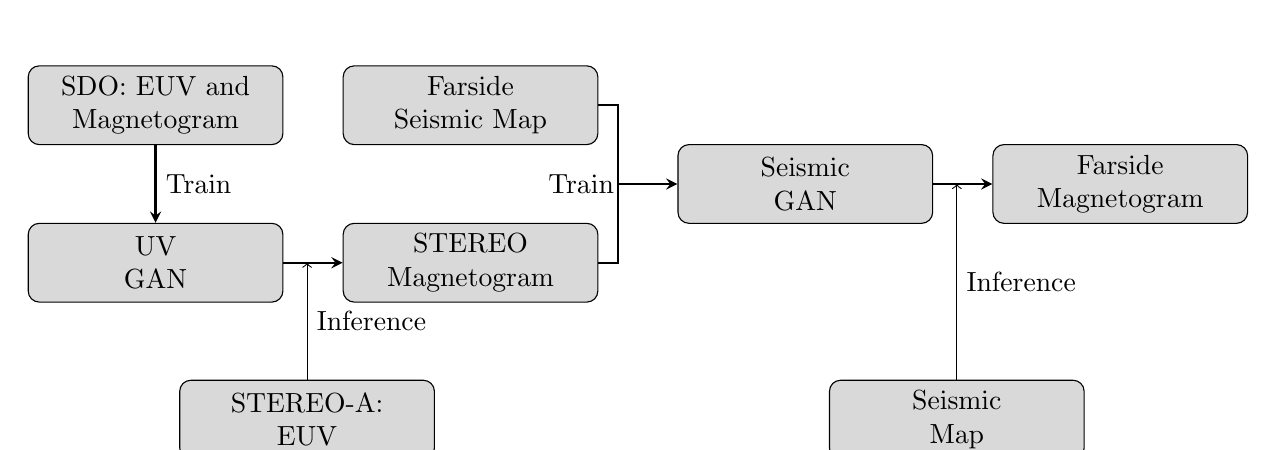
\begin{tikzpicture}[node distance=4cm]

      % \draw[help lines] (0,0) grid (10cm,10cm);

      \coordinate (T) at (5,4);

      \node (SGAN) [cool, right of=T, left=0.0cm] {Seismic\\ GAN};
  
      \node (SM) [cool, left of=T, above=1cm, right=0.5cm] {Farside\\ Seismic Map};
      \node (STEM) [cool, left of=T, below=1cm, right=0.5cm] {STEREO Magnetogram};

      \node (SDO) [cool, left of=SM] {SDO: EUV and \\ Magnetogram};
      \node (UVGAN) [cool, left of=STEM] {UV\\ GAN};
      
      % \node (E) [cool] {STEREO EUV image};
      
      \node (FM) [cool, right of=SGAN] {Farside\\ Magnetogram};

      \coordinate (I1) at ([xshift=0.3cm]UVGAN.east);

      \node (SUV) [cool, below of=I1, above=1.5cm] {STEREO-A:\\ EUV};
      \draw [->] (SUV) -- node[anchor=west] {Inference} (I1);

      \coordinate (I2) at ([xshift=0.3cm]SGAN.east);

      \node (SM2) [cool, below of=I2, above=0.5cm] {Seismic\\ Map};
      \draw [->] (SM2) -- node[anchor=west] {Inference} (I2);

      \draw [line] (STEM) -| (T);
      \draw [line] (SM) -| (T);
      \draw [arrow] (T) -> node[anchor=east, xshift=-0.3cm] {Train}(SGAN);

      \draw [arrow] (SDO) -> node[anchor=west] {Train}(UVGAN);
      \draw [arrow] (UVGAN) -> (STEM);
      \draw [arrow] (SGAN) -> (FM);

      % \coordinate (FF) at ([xshift=-1.5cm]F.west); % we collect the edges in front of Q
      % \coordinate (MM) at ([xshift=-1.5cm]M.west); % we collect the edges in front of Q
      
      % \draw [arrow] (D) -- node[anchor=south, text width=2cm] {Helioseismic Holography} (P);
      % \draw [arrow] (MM) -- node[anchor=south] {cGAN} (M);
      % \draw [line] (P) -|  (FF);
      % \draw [line] (M) -|  (FF);
      % \draw [line] (S) -|  (MM);
      % % \draw [line] (E) -|  (MM);
      % \draw [arrow] (FF) -- node[anchor=south] {cGAN} (F);

  \end{tikzpicture}
  \caption{A simplified diagram of the project pipeline. Nearside SDO
  EUV/magnetogram image pairs are used to train the `UV-GAN', which is then
  used to generate farside STEREO magnetograms. Farside seismic map/STEREO
  magnetogram pairs are then used to train the `Seismic-GAN' which can then be
  used to generate farside magnetograms from nearside seismic maps without the
  need for STEREO-A data.}
  \label{fig:simple_diagram}
\end{figure}



% , and full-disk dopplergrams which
% measure the line-of-sight motion of the solar surface. As detailed in Section
% \ref{sec:FHSM}, these dopplergrams can be used to generate farside seismic maps.
% However, by nature of orbiting the Earth, SDO is unable to image the solar
% farside except indirectly through farside helioseismic holography. Only three
% active solar probes, Parker Solar Probe, Solar Orbiter and Solar-Terrestrial
% Relations Observatory A (STEREO-A) measure the farside at any point in their
% orbit, and only STEREO-A consistently takes full-disk solar images. While
% STEREO-A does not produce magnetograms, the extreme ultraviolet imager onboard
% images the Sun at a wavelength of \SI{304}{\angstrom}. 


% However, not all hope is lost. The STEREO-A spacecraft is in a heliocentric
% orbit that traverses the Sun relative to the Earth, allowing it to observe the
% farside during some points of the orbit. While STEREO-A does not capture
% magnetograms of the Sun, it does take EUV images which can be used to create
% magnetograms by using a cGAN \citep{Kim2019}.\\

% A small complication is that no data is available from when STEREO-A was
% directly opposite the Earth (between March and July 2015), due to the
% interference from the Sun. This limits the ability to get magnetograms that
% exactly coincide with the farside seismic maps. To compensate for this, we can
% match farside seismic maps with images taken by STEREO-A at an earlier (later)
% time when it is behind (ahead of) the farside, such that the same `face' of the
% Sun is imaged due to its rotation. After generating the magnetograms from the
% STEREO-A EUV images, we can create a dataset of seismic maps with the
% corresponding magnetogram (albeit with some time difference).



% \begin{itemize}
%   \item This is essential, as the only currently reliable way of imaging the solar
%   farside is through farside helioseismic holography, with the generation of
%   farside seismic maps.
%   \item some research has been done on the correlation of seismic signatures and
%   magnetic field (https://iopscience-iop-org.ezproxy.lib.monash.edu.au/article/10.1086/521592)
%   \item research into detecting active regions from farside seismic maps ()
% \end{itemize}



% \begin{itemize}
%   \item While many Earth-based solar observatories exist, space-based
%   observatories can monitor the Sun without the limitation of
%   atmospheric absorption.
%   observing the Sun from the  Earth comes with many issues 
%   \item The best way to image the Sun is directly from space-based telescopes.
%   \item

%   Therefore, an indirect
%   measurement of the magnetic field must be employed to reliably predict extreme
%   space weather events.
  
%   \citet{Kim2019} trained an image-to-image cGAN to generate artificial
%   magnetograms from Extreme Ultraviolet (EUV) images. This training was done
%   using pairs of \SI{304}{\angstrom} EUV images and magnetograms from SDO. This
%   trained cGAN was then used to generate artificial farside magnetograms from
%   similar STEREO-A EUV images.

%   \item however, they used a saturation point of 100 Gauss, limiting the ability
%   to predict strong magnetic fields, especially considering that active regions
%   can have magnetic field strengths of thousands of Gauss

%   \item Furthermore, STEREO-A is currently on the nearside coming towards the Earth
%   and only has a partial view of the solar farside (see Figure
%   \ref{fig:stereo_pos}).

%   \item As such the only consistent observation of the Farside comes from
%   farside helioseismic holography.

%   \item To generate farside magnetograms from seismic images using an
%   image-to-image cGAN, we need to construct a dataset of seismic
%   image/magnetogram pairs. However, since we have no available farside
%   magnetograms, the creation of this dataset presents its own issue. To
%   overcome this issue, we first train an image-to-image cGAN to generate
%   magnetograms from \SI{304}{\angstrom} solar EUV images.

% \end{itemize}





%
%
%
%
\chapter{Data Preparation}
\label{chap:data}
%
%
%
%

To generate farside magnetograms from farside seismic maps, we first create two
distinct datasets
\begin{enumerate}
  \item a nearside dataset consisting of EUV and magnetogram image pairs, and
  \item a farside dataset consisting of seismic map and EUV image pairs.
\end{enumerate}
As detailed in Chapter \ref{chap:training}, the farside EUV images will be used
to generate magnetograms, which can then be used to train an image-to-image cGAN
to generate magnetograms from farside seismic maps. \\


To maximise the effectiveness of each cGAN, we need to make the images consistent
across each dataset such that the only differentiation between images is the
change in solar activity. Furthermore, in each image-to-image translation, we
need to ensure that the active regions are located in the same position in both the
input and output images. We must therefore account for the following effects
\begin{enumerate}[i]
  \item changes in time of image capture, 
  \item changes in location of image capture,
  \item the solar cycle in which the image was taken,
  \item the position of the Sun in images,
  \item the orientation of the Sun in images,
  \item the projection used in images,
  \item corrupted images or images with data artifacts,
  \item instrument degradation over time,
  \item instrument saturation, and
  \item the amplitude of pixel values between image data-sets.
\end{enumerate}
In this chapter we detail how we obtain the data and prepare it for training,
accounting for the above effects.

% \begin{itemize}
  
%   \item Nearside vs Farside (i.e. why we need it)
%   \item Data sources were:
%         \begin{itemize}
%           \item STEREO-A EUV images
%           \item SDO EUV images
%           \item SDO magnetograms
%           \item farside helioseismic holography maps
%         \end{itemize}
%   \item magnetograms measure the radial magnetic field, using filtegrams
%   \item % https://link.springer.com/content/pdf/10.1007/s11207-011-9834-2.pdf
%   \item figure showing positions and trajectory of stereo, sun Earth, SDO and
%         imaginary satellite for acoustic maps
%   \item figure (maybe the same one) showing plot of stereo position in
%   \item position data from http://www.srl.caltech.edu/STEREO/docs/position.html
%   \item This is in Heliocentric Earth equatorial (HEEQ): This system has its Z
%         axis parallel to the Sun's rotation axis (positive to the North) and its X
%         axis towards the intersection of the solar equator and the solar central
%         meridian as seen from the Earth. This system is sometimes known as
%         heliocentric solar (HS)
% \end{itemize}



\section{Data Collection}
\label{sec:data_collection}
As detailed in Section \ref{sec:outlook}, our research required data from the
Solar Dynamics Observatory (SDO) and the Solar Terrestrial Relations Observator A
(STEREO-A) in addition to farside seismic maps.
% created using SDO dopplergrams.
% \begin{enumerate}
%   \item SDO EUV images,
%   \item SDO magnetograms,
%   \item STEREO-A EUV images, and
%   \item helioseismic holography maps.
% \end{enumerate}
% EUV images with a wavelength of \SI{304}{\angstrom} are produced by both the SDO
% and STEREO-A EUV telescopes and were therefore chosen for this project. As explained in
% Section \ref{sec:Sun}, light at \SI{304}{\angstrom} is emitted by the
% chromosphere - the atmospheric layer above the photosphere. \\
As SDO is orbiting the Earth, both the SDO EUV images and magnetograms were
taken of the nearside. STEREO-A is instead in a heliocentric orbit, with an
orbital period of 346 days. As such, it has rotated about the Sun relative to
the Earth taking parital images of the farside throughout its 14-year life.
Finally, the seismic maps are generated from SDO dopplergrams and image the
farside of the Sun as detailed in Section \ref{sec:FHSM}. \\

Of particular importance when collecting the data is the time and location of
the image capture. Here we detail what decisions were made in regards to these
factors.

% Changes in time of image capture
% Changes in location of image capture
% The solar cycle in which the image was taken


\subsection{Nearside Data}
As all the nearside data comes from SDO, the position of the telescope does not
change between data types. Furthermore, SDO captures EUV images and magnetograms
with a cadence of 12 and 45 seconds respectively, allowing us to compare these
with very little time difference. The images were provided by the Joint Science
Operation Centre\footnote{See \url{http://jsoc.stanford.edu}} and were
collected every 12 hours between April 2010, when the first SDO data became
available, and December 2019 - the end of Solar cycle 24. Since all data was
taken during this solar cycle, we did not have to take into account the flipping
of the global magnetic field which occurs between solar cycles (see Section
\ref{sec:dynamo}). Due to a combination of missing or poor quality images (see
Section \ref{sec:Data prep}) this process resulted in a total of 4247 nearside
EUV/magnetogram pairs. While the nearside data was taken from only a single data
source (SDO), making the data collection relatively simple, this is not the case
for the farside data.

\subsection{Farside Data}
Unlike the nearside data, our farside data comes from two separate sources.
STEREO-A provides the farside EUV images, while the SDO provides the
dopplergrams that are used to generate the farside seismic maps. Complicating
matters further, for the majority of its mission STEREO-A is not directly
facing the farside and only has a partial view. Furthermore, STEREO-A experienced
reduced telemetry rates between August 2014 and January 2016, with complete
instrument shut off between March and July 2015 due to STEREO-A's superior
solar conjunction \citep{ossing_stereo_2017}. Figure \ref{fig:stereo_pos} shows
the trajectory of STEREO-A relative to the Earth with the points of reduced or no
telemetry indicated. \\

To overcome this limitation, we can leverage the rotation of the Sun and compare
farside seismic maps to STEREO-A images with a time delay, such that both images
capture the same `face' of the Sun. For example, if STEREO-A imaged the Sun while
\SI[]{45}[]{\degree} from the solar farside, after approximately 3 days the Sun
would have rotated such that the same face of the Sun would now be on the
farside, and could be imaged by farside helioseismic holography. By using such a
method, we can effectively compare farside seismic maps with not-quite-farside
STEREO-A EUV images. This method isn't perfect however and has two obvious drawbacks
\begin{enumerate}
  \item the differential rotation of the Sun means that active regions won't
  necessarily be in the same position after a time delay, and
  \item active regions are constantly changing, for example, the emergence of
  active regions can take place over hours or days, while the decay of
  sunspots may last from days to weeks
  \citep{van_driel-gesztelyi_evolution_2015}.
\end{enumerate}
These limitations will be further discussed in Chapter \ref{chap:discussion}. \\

To implement this correction, we must first determine the rotational rate of the
Sun. As can be seen from Figure \ref{fig:butterfly diagram}, the majority of the
active regions in solar cycle 24 are at latitudes between $\pm
\SI{30}{\degree}$. Furthermore, the rotation of the Sun is roughly homogeneous
at these latitudes, with the frequency of rotation varying between \SI{425}{nHz}
and \SI{450}{nHz} (see Figure \ref{fig:solar_rotation}). We chose to estimate
this rotation rate based on the Carrington rotational period of
\SI{27.2753}{days}. This corresponds to the average synodic rotational period of
sunspots, or equivalently, the synodic solar rotation at a latitude of
approximately \(\SI[]{26}[]{\degree}\) \citep{carrington_observations_1863}. It
should be noted that the synodic rotation is measured relative to the Earth (and
therefore the solar farside). An appropriate choice of coordinates for the
correction calculations is therefore the heliocentric Earth equatorial
coordinate system. In these coordinates, the $z$-axis is aligned with the axis
of solar rotation, while the $x$-axis points from the centre of the Sun to the
Earth (see again Figure \ref{fig:stereo_pos}). The time delay between a STEREO-A
image and the farside is then given by
\begin{align}
  \Delta t(t_s) = \left(\frac{\theta(t_s)}{2\pi}\right)T \, ,\\
  \intertext{with}
  \theta(t_s) = \arctan{\left(\frac{y(t_s)}{x(t_s)}\right)} \, ,
\end{align}
where $T$ is the aforementioned Carrington rotational period, $\theta(t_s)$ is
the angle between STEREO-A and the solar farside, and $(x(t_s), y(t_s))$ is the
position of STEREO-A at time $t_s$ in heliocentric Earth equatorial coordinates.
It should be noted that $\theta(t_s)$ and therefore $\Delta t$ are negative
while STEREO-A is `behind' the solar rotation, and positive while STEREO-A is
`ahead' of the solar rotation. We can therefore calculate the equivalent farside
time ($t_f$) for a given $t_s$ as follows
\begin{align}
  t_f = t_s - \Delta t(t_s) \, .
\end{align}
This was used to calculate the `farside equivalent' time at each point in
STEREO-A's orbit, using STEREO-A position data provided by the Space Radiation
Lab at California Institute of Technology\footnote{See
\url{www.srl.caltech.edu/STEREO}.}. \\

The Joint Science Operation Centre has been producing farside seismic maps with
a cadence of 12 hours since April 2010\footnote{See
\url{jsoc.stanford.edu/data/farside/Phase_Maps}.}. For each of these images, the
equivalent time for STEREO-A was calculated and the \SI{304}{\angstrom} EUV image
that best matched this time was found. If the image time disagreed with the
ideal time by more than 2 hours the image was discarded. As STEREO-A produces
\SI{304}{\angstrom} EUV images with a cadence of \SI{10}{minutes} this only
affected images produced during periods of reduced telemetry. The remaining
images were downloaded from the Virtual Solar Observatory\footnote{See
\url{virtualsolar.org}.}. \\

With the dataset of images obtained, we now turn our attention to ensuring
consistancy between images.
% However, before using these images we need to ensure that the Sun is represented
% consistently across each dataset such that any solar features appear in the
% same location.

\begin{figure}[ht]
  \centering
  \includegraphics[width = 0.7\linewidth]{STEREO_pos.pdf}
  \caption[STEREO-A Trajectory]{Trajectory of STEREO-A between October 2006 and January 2021 in the
  Heliocentric Earth Equatorial coordinate system. In these coordinates, the Sun
  is at the origin with the Earth fixed on the $x$-axis. Each `bump' in STEREO's
  Trajectory correspond to a year on Earth. \textit{Image generated using
  data provided by the Space Radiation Lab at California Institute of Technology.}}
  \label{fig:stereo_pos}
\end{figure}


\section{Image Projections}
\label{sec:proj}
% Position of the sun in images
% Orientation of the Sun in images
% Projection used in image
To ensure consistency between image datasets we need to take into account the
position and orientation of the Sun as well as how the Sun is represented on
each image. As there are many ways to project three-dimensional data onto a
two-dimensional image, consistent representation of the Sun is not guaranteed.
Therefore to effectively compare different images of the Sun we must take into
account the projection used to construct the image.

\subsection{Nearside Data}
Both SDO EUV images and magnetograms use the same projection. For
these images, each pixel directly corresponds to a pixel on the camera sensor,
which in the case of SDO and STEREO-A images is a charge-coupled device or
CCD \citep{kaiser_stereo_2008,lemen_atmospheric_2012}. As the CCD is a flat plane,
the resultant image is a projection of the Sun onto the parallel tangent plane of the
celestial sphere.
% gnomonic projection
For both SDO and STEREO-A, the angle subtended by the solar disk is
approximately \SI[]{0.5}[]{\degree} and so we can instead approximate the image
to be projected against the celestial sphere itself. This is a very good
approximation, and at a distance of 1 AU (approximately the orbital radius of
SDO and STEREO-A), the angles describing the Sun on the tangent plane match the
angles on the celestial sphere to at least five significant figures
\citep{thompson_w_t_coordinate_2006}. This projection is known as a
helioprojective-cartesian projection, and measures positions in terms of the
longitude \(\theta_x\) and latitude \(\theta_y\) of the celestial sphere.\\

SDO Magnetograms are taken by the Helioseismic and Magnetic Imager
\citep{scherrer_helioseismic_2012}, while the EUV images are taken by the
Atmospheric Imaging Assembly \citep{lemen_atmospheric_2012}. To account for the
difference in orientation of these two instruments, the images were rotated such
that the uppermost section of each image corresponded to the northernmost region
of the solar disk. To find the suitable angle of rotation, the helioprojective
latitude and longitude were found for each pixel using image metadata.
Furthermore, the distance to the Sun changes throughout SDO's orbit due to the
eccentricity of the Earth, changing the relative size of the solar disk. To
remove this discrepancy, while also removing unnecessary pixels, the images were
cropped to the radius of the Sun, again using information extracted from the
image metadata. This process was more complex for the farside data.

% not sure if I want to keep it like this or change it to below:
%   \item Fortunately both EUV and magnetogram images are taken by SDO at very similar
%   times, and both sets of images are projected into helioprojective-cartesian
%   coordinates.
%   \item In this coordinate system, observations are projected against the
%   celestial sphere, and positions are measured in the longitude \(\theta_x\) or
%   latitude \(\theta_y\) of the celestial sphere, with the centre of the disk
%   (i.e. the point of the Sun closest to the observer) at the origin.
%   \item Note: this is not exactly correct, as the camera sensor (in this case a
%   CCD detector) is a flat plane. As such, we are actually projecting on to a
%   tangent plane of the celestial sphere (gnomonic projection). However since the
%   angle subtended by the solar disk is \(\approx \SI[]{0.3}[]{\degree} \), this
%   can be accurately approximated as a helioprojective projection. In fact, at a
%   distance of 1 AU (approximately the orbital radius of SDO and STEREO), the
%   angles on the tangent plane are the same as the angles on the celestial sphere
%   to at least five significant figures \cite{thompson_w_t_coordinate_2006}
%   \item The helioprojective latitude and longitude of each pixel on the EUV and
%   magnetogram images could be found using the metadata from each image.
%   \item The instruments used to create these images are rotated relative to each
%   other.

\subsection{Farside Data}
While the STEREO-A EUV data uses the same helioprojective-cartesian projection
as the nearside SDO data, this is not the case for the farside seismic maps. The
seismic maps instead use a Carrington heliographic projection, where positions
are measured in solar latitude (\(\Theta\)) and Carrington longitude
(\(\Phi_c\)). This coordinate system rotates with the Sun such that the prime
meridian of these coordinates faces the Earth approximately every 27
days\footnote{To be precise, the prime meridian rotates such that it aligns with
the solar central meridian (according to an observer on the Earth) once every
Carrington rotation (27.2753 days).}. To directly compare STEREO-A EUV images
with farside seismic maps we must therefore re-project the seismic maps into
helioprojective-cartesian coordinates. \\

To transform the seismic maps, we need to find the points in the original
heliographic projection that correspond to each pixel in the final
helioprojective image. In general, these points will not directly correspond to
the centre of a pixel and so we must first apply an image interpolation method
to construct a continuous version of the original heliographic image. To find
these points we use an intermediate transformation to heliocentric-cartesian
coordinates, i.e. 
\begin{align*}
  \text{Helioprojective-cartesian} \rightarrow \text{Heliocentric-cartesian} \rightarrow \text{Carrington Heliographic} \, .
\end{align*}
Heliocentric-cartesian coordinates give the true spatial position of an object
($x$, $y$, $z$) with the origin at the centre of the Sun, the z-axis pointed
toward the observer and the y-axis in the plane containing the z-axis and the
rotational axis of the Sun. The x-axis is oriented such that all three axes
create an orthogonal right-handed coordinate system. \\


To convert helioprojective-cartesian coordinates into heliocentric-cartesian
coordinates, we use the following transformation, provided by
\citet{thompson_w_t_coordinate_2006}:
\begin{align}
  x &= d \cos \theta_y \sin \theta_x \, , \\
  y &= d \sin \theta_y \, \text{and} \\
  z &= D_\odot - \cos \theta_y \cos \theta_x \, .
  \label{eqn:heliop_to_helioc}
\end{align}
Where \(d\) is the distance between the observer and the point being observed,
and \(D_\odot\) is the distance between the observer and the centre of the Sun.
After some trigonometry, it can be shown that if the point being observed is on
the surface of the Sun, then
\begin{align}
  d &= D_0 \cos\theta - \sqrt{D_\odot^2 \left( \cos^2\theta - 1 \right) + R_\odot } \, , \\
  \intertext{where}
  \theta &= \cos^{-1}\left(\cos\theta_y \cos\theta_x \right) \, .
\end{align} \\

Similarly, we can convert from heliocentric-cartesian coordinates to Carrington heliographic
coordinates as follows:
\begin{align}
  \Theta &= \sin^{-1}\left( \frac{y \cos B_0 + z \sin B_0}{r}\right) \, , \\
  \Phi_c &= \arg (z \cos B_0 - y \sin B_0, x) + \Phi_{0} \,
  \intertext{where}
  r &= \sqrt{x^2 + y^2 + z^2} \, ,
\end{align}
and \(B_0\) and \(\Phi_{0}\) are the Carrington heliographic latitude and
longitude of the Observer. \\


Since we are directly comparing the seismic maps to STEREO-A EUV images, we
choose values \(B_0\), \(\Phi_0\) and \(D_\odot\) according to an observer at
STEREO-A, with the longitude adjusted to be opposite the Earth (i.e. the centre
of the farside). These exact values were obtained from the STEREO-A image
metadata. The seismic maps were re-projected using this transformation with
bi-linear interpolation. Figure \ref{fig:projection} shows a seismic map before
and after this transformation. \\
%TODO: overlay stereo and seismic maps or at least show stereo as well. Also
%maybe inbetween image

The STEREO-A EUV images were then prepared in the same manner as the nearside
data, by first rotating then cropping the images. This step was not required for
the re-projected seismic maps, as they were already correctly aligned as a
by-product of the transformation. With all images correctly aligned, it is now
necessary to take into account effects from the individual imaging instruments.

\begin{figure}[t]%
  \centering
  \subfigure[]{%
    \label{fig:heliographic}
    \includegraphics[height=2in]{heliographic.png}%
  }%
  \qquad
  \subfigure[]{%
    \label{fig:helioprojective}%
    \includegraphics[height=2in]{helioprojective.png}% 
  }%

  \caption[]{\subref{fig:heliographic} An original seismic map with a
  heliographic-cartesian projection. \subref{fig:helioprojective} The same
  seismic map after projection into helioprojective-cartesian coordinates.}
  \label{fig:projection}
\end{figure}



\section{Data Preprocessing}
% Amplitude of pixel values between image data-sets
% Instrument degradation over time
% Instrument clipping
% Corrupted images or images with data artifacts

\label{sec:Data prep}
Before using the images we need to account for various factors and
inconsistencies in the imaging process. Of particular importance is the EUV data
which comes from two data sources: SDO and STEREO-A. To use data from both
sources interchangeably, we must make the images consistent between these
datasets.

\subsection{Extreme Ultraviolet Data}
\label{sec:UV_prep}
As mentioned in Section \ref{sec:proj}, STEREO-A and SDO both use a CCD to image
the Sun at a wavelength of \(\SI[]{304}[]{\angstrom}\). Each pixel in the CCD
converts the incoming photons into an electric charge, which is subsequently
measured. The value of each pixel in units of digital number (DN), is given by
the integral 
\begin{align}
  \label{eqn:pixel value}
  p(\bm{x}) = \int_0^\infty \eta(\lambda) \int_{\text{pixel } \bm{x}} I(\lambda, \bm{\theta}) d\bm{\theta} d\lambda\, ,
\end{align}
were $I(\lambda, \bm{\theta})$ is the spectral radiance of pixel $\bm{x}$ at point
$\bm{\theta}$ and wavelength $\lambda$, and $\eta(\lambda)$ represents the efficiency
of the \SI{304}{\angstrom} channel in the telescope, measured in units of
DN per unit flux \citep{boerner_initial_2012}. Informally,
$\eta(\lambda)$ is equivalent to the ratio of the signal strength (in DN) of the
CCD to the total electromagnetic flux at wavelength $\lambda$ incident on pixel
$\bm{x}$. As we are attempting to measure the flux at \SI{304}{\angstrom},
$\eta$ would ideally be large for wavelengths close to
\SI{304}{\angstrom}, vanishing as we move away from this wavelength.
Approximating $\eta$ to be zero for $\lambda \neq \SI{304}{\angstrom}$, Equation
\ref{eqn:pixel value} reduces to
\begin{align}
  p(\bm{x}) &= \eta(\SI{304}{\angstrom}) \int_{\text{pixel } \bm{x}} I(\SI{304}{\angstrom}, \bm{\theta}) d\bm{\theta} \\
  \intertext{and so,}
  p(\bm{x}) &\propto \Phi(\bm{x}, \SI{304}{\angstrom}) \, , \label{eqn:pixel propto flux}
  \intertext{where}
  \Phi(\bm{x}, \lambda)& = \int_{\text{pixel } \bm{x}} I(\lambda, \bm{\theta}) d\bm{\theta}
\end{align}
is the electromagnetic flux at wavelength $\lambda$ incident on pixel $\bm{x}$.
And so we find our pixel values are linearly proportional to the
EUV flux to a reasonable approximation.\\


Each raw image is processed to remove data artifacts caused by the imaging,
and the resulting image is then made available for use. This image processing is
not perfect however, and we still have make some corrections ourselves before we
are ready to use the images.\\

From the 4313 SDO EUV images used between 2010 and 2020, the pixel values for
the AIA data range from \(\SI[]{-166}[]{DN}\) to \(\SI[parse-numbers=false]{2^{14} - 1}[]{DN}\). To get
a handle on this data, a range of the pixel value percentiles were calculated
for each image. Figure \ref{fig:aia_percentiles} shows these percentiles plotted
as a function of time. Corrupted or otherwise poor quality images could then be
identified due to the large irregularity in the percentiles of those images, as
can be seen in Figure \ref{fig:aia_outliers}. After reviewing the offending
images, a simple threshold was used to remove the outliers.\\

Also apparent from Figure \ref{fig:aia_outliers} is the decreasing exposure of
the images between 2010 and 2020. This is consistent with the degradation of the
SDO's \SI{304}{\angstrom} EUV channel found by \citet{boerner_photometric_2014}.
Figure \ref{fig:aia_degradation} shows a comparison in the exposures of images
taken in 2011, 2015 and 2019 respectively, in which the reduced exposure can be
seen. To account for this, the pixel values of each image were given a weighting
factor depending on the time the image was taken, i.e.
\begin{align}
  p_f = w(t) p_i \, ,
\end{align}
where $p_i$ is the initial pixel value, $p_f$ is the final pixel value and $w(t)$
is the weighting factor at time $t$. The weighting factor was chosen to be the 
reciprocal of a 50-point rolling average of the 75th
percentile at time $t$, i.e.
\begin{align}
  w(t) = \frac{1}{\sum\limits_{i=-25}^{25}P_{75}(t + i \Delta t)} \, ,
\end{align}
where $P_{75}(t)$ is the 75th percentile pixel value of the image taken at time
$t$, and $\Delta t$ is the time between images, in our case 12 hours. The 75th
percentile was picked as it had the lowest 50-point relative variance of the
percentiles calculated. This indicated that the 75th percentile was more
indicative of the background Sun as opposed to individual active regions, and
would therefore better capture the degradation of the instrument over time. It
should be noted however that the 75th percentile was still affected by the solar
activity, and some of this information was inadvertently removed in this
process. This did not affect our inferences, but will be discussed further in
Chapter \ref{chap:results_and_analysis}. The percentiles of the data after
applying this weighting are shown in Figure \ref{fig:aia_no_degradation}. \\

To ensure consistency between the two EUV datasets, we need to normalise and
correct the STEREO-A data in the same method as the SDO data. Figure
\ref{fig:stereo_percentiles} shows the initial percentiles of pixel values for
the STEREO-A data, with the times of reduced and no telemetry resulting in the
large gap in the dataset. Once again, poor quality images could be identified by the
large deviations in the percentile values and were removed using a simple
cutoff criterion (see Figure \ref{fig:stereo_outliers}).\\

It was found that approximately $3 \%$ of the pixels in the SDO data had a value
below 0, while the same percentage of pixels from STEREO-A images had a value
below $\SI[]{725}[]{DN}$. Accordingly, the STEREO-A pixels were decreased by
$\SI[]{725}[]{DN}$ before dividing by the rolling average of the 75th
percentile. Figure \ref{fig:stereo_no_degradation} shows the pixel value
percentiles of the STEREO-A images after this process. At this stage in the
normalisation process both SDO and STEREO-A datasets had approximately $3 \%$ of
the data had a value below \SI{0}{DN}, and $75 \%$ of the data with a value
below \SI{1}{DN}. As the pixel values are (approximately) linearly proportional
to the EUV flux (see Equation \ref{eqn:pixel propto flux}), these two points are
enough to constrain the two datasets such that a given pixel value will
correspond to the same level of EUV flux for images in either dataset taken
at roughly the same time. \\
% Assuming that the 75th percentile is the same (flux) at that time.

One last discrepancy between the two datasets is the saturation points at which
the CCD cannot record any value above. While both instruments initially have a
saturation point at $ \sim \SI[parse-numbers=false]{2^{14}}[]{DN}$ (see Figures
\ref{fig:aia_percentiles} and \ref{fig:stereo_data_prep}), this has been
distorted during our image processing, as can be seen in Figures
\ref{fig:aia_no_degradation} and \ref{fig:stereo_no_degradation}. To make this
consistent between the STEREO-A and SDO images, we introduce our own artificial
saturation point. To choose this upper bound, we found the minimum of a 50
rolling average of the 100th percentile of pixel value for the STEREO-A data,
which was \SI[]{32}[]{DN}. The upper bound can be seen in Figure
\ref{fig:stereo_no_degradation}. To avoid losing information about regions of
intense solar activity, it was important to make this upper bound as high as
possible while keeping the two datasets consistent. This constraint did not
apply to a lower bound, which was chosen to have a value of \SI{0}{DN}. Both
datasets were normalised by dividing by the upper bound such that all pixels had
a value between 0 and 1. The STEREO-A and SDO datasets appeared consistent after
normalisation as can be seen in Figure \ref{fig:sdo_stereo_comparison}. Furthermore,
the general trend of the solar cycle was retained despite the normalisation
process, with solar activity peaking in 2014. We now turn to the Magnetogram and
seismic data.



\begin{figure}[t]%
  \centering
  \subfigure[]{%
    \label{fig:aia_2011}%
    \includegraphics[height=1.5in]{AIA_2011.01.01_00:00:00.png}% 
  }%
  \qquad
  \subfigure[]{%
    \includegraphics[height=1.5in]{AIA_2015.01.01_00:00:00.png}%
    \label{fig:aia_2015}%
  }%
  \qquad
  \subfigure[]{%
    \includegraphics[height=1.5in]{AIA_2019.01.01_00:00:00.png}%
    \label{fig:aia_2019}%
  }%
  \caption[]{Images taken by SDO AIA $\SI[]{304}[]{\angstrom}$ on the first of January in 2011
    \subref{fig:aia_2011}, 2015 \subref{fig:aia_2015} and 2019
    \subref{fig:aia_2019}. Due to the degradation of the instrument, the
    exposure reduces over time. \textit{Images courtesy of NASA.}}
  \label{fig:aia_degradation}
\end{figure}


\begin{figure}[t]%
  % \centering
  \subfigure[]{%
    \label{fig:aia_percentiles}
    \includegraphics[width=\linewidth]{AIA_percentiles.png}%
  }%
  \qquad
  \subfigure[]{%
    \label{fig:aia_outliers}%
    \includegraphics[width=\linewidth]{AIA_outliers.png}% 
  }%
  \qquad
  \subfigure[]{%
    \label{fig:aia_no_degradation}%
    \includegraphics[width=\linewidth]{AIA_no_degradation.png}% 
  }%

  \caption[]{\subref{fig:aia_percentiles} The percentiles of the SDO
  \SI{304}{\angstrom} EUV data for images taken every 12 hours between May 2010
  and December 2019. Due to the large range of data, the 25th to 100th
  percentiles were plotted on a log scale. \subref{fig:aia_outliers} The 75th
  percentile of the SDO EUV data. A simple threshold was used to remove poor
  quality data. \subref{fig:aia_no_degradation} The percentiles of the SDO
  EUV data after accounting for instrument degradation.}
  \label{fig:aia_data_prep}
\end{figure}


\begin{figure}[t]%
  % \centering
  \subfigure[]{%
    \label{fig:stereo_percentiles}
    \includegraphics[width=\linewidth]{STEREO_percentiles.png}%
  }%
  \qquad
  \subfigure[]{%
  \label{fig:stereo_shifted}
  \includegraphics[width=\linewidth]{STEREO_shifted.png}%
}%
\qquad
\subfigure[]{%
\label{fig:stereo_outliers}
\includegraphics[width=\linewidth]{STEREO_outlier.png}%
}%
\qquad
\subfigure[]{%
\label{fig:stereo_no_degradation}
\includegraphics[width=\linewidth]{STEREO_no_degradation.png}%
}%
  
  \caption[]{\subref{fig:stereo_percentiles} The percentiles of the STEREO-A
  \SI{304}{\angstrom} EUV data for images taken every 12 hours between January 2010
  and December 2019. The gap in the data is due to the loss of data during the
  STEREO-A solar conjunction. \subref{fig:stereo_outliers} The 75th
  percentile of the STEREO-A EUV data. A simple threshold was used to remove poor
  quality data. \subref{fig:stereo_no_degradation} The percentiles of the
  STEREO-A EUV data after accounting for instrument degradation. The dashed
  horizontal line indicates the point above which data was clipped to ensure
  consistent saturation.}
  \label{fig:stereo_data_prep}
\end{figure}


\begin{figure}[t]
  \centering
  \includegraphics[width=\linewidth]{AIA_STEREO_normalised.png}
  \caption{Comparison of the SDO and STEREO-A EUV data after normalisation.}
  \label{fig:sdo_stereo_comparison}
\end{figure}



\subsection{Magnetogram and Seismic Data}
We show the percentiles of pixel values from the SDO magnetogram data in Figure
\ref{fig:hmi_p}. Each pixel on a magnetogram image measures the average
line-of-sight magnetic field ($\mathbf{B}\cdot\mathbf{\hat{r}}$) in units of
Gauss (G) on the surface of the Sun subtended by the pixel. Similarly, Figure
\ref{fig:seismic_p} shows the percentiles of pixel values for the seismic maps.
As explained in Section \ref{sec:HSM}, seismic maps measure the relative phase
shift experienced by p-modes as they travel to and from the solar farside. \\

Fortunately, neither of these datasets exhibited the instrument degradation or
image saturation seen in the EUV data. The magnetogram data was normalised by
dividing it by the absolute maximum pixel value across all the data, which in
this case was $\SI[]{5847.6}[]{G}$, limiting the pixel values to between $-1$
and $1$. Importantly this process is completely reversible, with information
loss only from rounding errors. The raw seismic data had a range between
\SI{-0.9}{Rad} and \SI{0.8}{Rad}. As such normalising this data was deemed
unnecessary. %TODO: explain WHY we need the normalisation
With our data prepared and normalised we now turn to training each of the
image-to-image cGANs.

\begin{figure}[t]%
  % \centering
  \subfigure[]{%
    \label{fig:hmi_p}
    \includegraphics[width=\linewidth]{HMI_percentiles.png}%
  }%
  \\
  \subfigure[]{%
  \label{fig:seismic_p}
  \includegraphics[width=\linewidth]{phase_percentiles.png}%
}%
  \caption[]{\subref{fig:hmi_p} shows the percentiles of the pixel values for
  the magnetogram data. \subref{fig:seismic_p} shows the percentiles of pixel
  values for the seismic data.}
  \label{fig:hmi_seismic_p}
\end{figure}


%
%
%
%
%
%
%
%
\chapter{Training}
\label{chap:training}
%
%
%
%
%
%
%
%
With our data processing done, we are finally ready to begin training our deep
neural networks.
% - both the UV-GAN and seismic GAN
%TODO make it a story.
%TODO fix this -- maybe introduce UV-GAN and Seismic-GAN earlier.
We require two deep neural networks to generate farside magnetgorams from
seismic maps. The first of these must generate magnetograms from EUV
\SI{304}{\angstrom} images, which can then be used to generate `STEREO
Magnetograms' from our STEREO-A EUV data. The second network must then generate
magnetograms from seismic maps. In both cases, we use an image-to-image cGAN,
which has proven to be very effective at image-to-image translation. We
henceforth refer to these two cGANs as the `UV-GAN' and the `Seismic-GAN'
respectively. As outlined in Section \ref{sec:cgan}, each of these cGANs consist
of two competing networks: a `generator' and a `discriminator'. The same
generator and discriminator architecture is used for both the UV-GAN and the
Seismic-GAN. In this chapter, we outline the architecture used for the UV and
Seismic-GAN and describe how these deep neural networks were trained.



% \begin{itemize}
%   \item the process for creating a network capable of producing farside
%   magnetograms from seismic maps consists of three parts.
%   \begin{enumerate}
%     \item The UV-GAN is trained to generate magnetograms from uv images by using
%     SDO UV/Magnetogram image pairs
%     \item The now trained UV-GAN is used to generate `STEREO' magnetograms from
%     STEREO-A UV images
%     \item The Seismic-GAN is trained to generate magnetograms from Seismic
%     images using STEREO-A magnetogram/ farside seismic image pairs.
%   \end{enumerate}
  
%   \item The same network model was used for parts 1. and 3., which consisted of
%   a U-NET style generator, and a fully convolutional discriminator. Figure
%   \ref{fig:solar_gans_diagram} shows a diagram of both GANs. This architecture
%   for each GAN was based on the one used by \citet{Kim2019} for a very similar
%   purpose.
% \end{itemize}

\begin{figure}
  \centering
  \centering
  \subfigure[]{%
    \label{fig:uv_GAN_diagram}%
    \includegraphics[width=\linewidth]{UV-GAN.pdf}% 
  }\\
  \subfigure[]{%
    \label{fig:seismic_GAN_diagram}%
    \includegraphics[width=\linewidth]{Seismic-GAN.pdf}% 
  }
  \caption{\subref{fig:uv_GAN_diagram} A diagram of the UV-GAN. The generator network
  attempts to create a synthetic magnetogram based on SDO EUV images, while the
  discriminator network attempts to determine if a given input was a true magnetogram,
  based on the same EUV image. At each iteration, an SDO EUV/magnetogram pair is
  passed through the UV-GAN, and the descriminator updates the networks.
  \subref{fig:seismic_GAN_diagram} A diagram of the Seismic-GAN. The seismic-GAN
  operates similar to the UV-GAN except that the inputs are a seismic image and
  a STEREO magnetogram - itself generated by the UV-GAN.}
  \label{fig:solar_gans_diagram}
\end{figure}

%
%
%
%
%
\section{Architecture}
%
%
%
%
%
%

The architecture for each cGAN was based on the one used by \citet{Kim2019}. In
their paper, they describe a cGAN similar to the UV-GAN we train which generates
magnetograms from EUV solar images. However, while the cGAN used by
\citet{Kim2019} was only capable of predicting magnetic field strengths of at
most 100 G, ours does not have this issue. Our model consists of a U-net style generator network
\citep{ronneberger_u-net_2015}, and a fully convolutional discriminator network. Figure
\ref{fig:solar_gans_diagram} shows a diagram of each cGAN.


\subsection{Generator}
The generator network must be capable of translating the conditional image
(either an EUV image or seismic map) into a magnetogram. For this purpose, we
chose a U-net \citep{ronneberger_u-net_2015}. U-nets were originally developed
for biomedical image segmentation, however have been used in a wide range of
astrophysics applications (for example
\citet{felipe_improved_2019,bekki_quantifying_2021,baso_solar_2019}). U-nets
consist of a downsampling path where the width and height of each layer are
reduced at each step, followed by an upsampling path where the width and height
increase at each step until reaching the original size. Many `skip
connections' join layers of the same size at either side of the `U'. The model used
in this work is shown in Figure \ref{fig:gen_model}. By implementing a U-net the
generator can perform image-to-image translation that retains the shape and
large scale structures of the input image while still capturing complex
relationships between the input and output. While the generator network must be
able to translate between image types, the discriminator network must be able to
evaluate the quality of its input.

  \begin{figure}
    \centering
    \includegraphics[width=\linewidth]{unet.pdf}
    \caption{Diagram of the generator network. The input is a ($1024\times
      1024$) image. At each step in the downsampling path, convolution, leaky ReLU
      activation and batch normalisation is applied until reaching a layer with
      size $(1\times 1\times 512)$. At each step in the upsampling path,
      convolution, cropping and batch normalisation are applied.
      % TODO need to explain these especially relu
    }
    \label{fig:gen_model}
  \end{figure}


\subsection{Discriminator}
The discriminator network is given two inputs: a magnetogram (either real or
generated) and the corresponding conditional image - an EUV image for the UV-GAN
or a seismic map for the Seismic-GAN. The network then attempts to determine if
the magnetogram input is real, based on the conditional image. The architecture
of the discriminator network we used is shown in Figure~\ref{fig:discrim_model}.
The output of the discriminator is a ($126\times 126$) array, where each element
has a value between 0 and 1. The training objective of the discriminator network
is to maximise its output for a true magnetogram input, and minimise its input
for a generated magnetogram input. A `perfect' descrimnator would then output an
array of only $0$'s for a fake magnetogram input, and an array of $1$'s for a
true magnetogram. On the other hand, the training objective of the generator is
to increase the error rate of the discriminator. Informally, the generator can be
thought of as trying to `fool' the discriminator into thinking that the magnetogram
it generated is real. Similar to Section \ref{sec:gan}, the discriminator's cost
function is given by
\begin{align}
  C_{D(Real)} &= -\mathds{E}\left[\log(D(\mathbf{x}|\mathbf{c}))\right]
\end{align}
for a `true' magnetogram input, and
\begin{align}
  C_{D(Fake)} &=  -\mathds{E}\left[\log(\mathds{1} -  D(G(\mathbf{c})|\mathbf{c}) ) \right]\,,
\end{align}
for a `fake' magnetogram input where $\mathbf{c}$ is the `conditional' input,
$D(\dotsb|\mathbf{c})$ is the discriminator output with a real ($\mathbf{x}$) or
fake ($G(\mathbf{c})$) magnetogram as an input, and $\mathds{1}$ is a tensor
full of $1$'s with the same shape as $D(\dotsb)$. The `log' is taken
element-wise in each expression, before the mean of all tensor elements is
taken. The total discriminator cost function is then
\begin{align}
  C_{D} = C_{D(Real)} + C_{D(Fake)} \,. \label{eqn:d_loss}
\end{align}
\par
As detailed in Section \ref{sec:cgan}, the discriminator also provides the cost
function for the generator. Unlike \ref{sec:cgan} an additional term was added
to minimise the absolute difference between the real and fake magnetograms. With
this addition, the generator cost function used was
\begin{align}
  C_{G} = -\mathds{E}\left[\log(D(G(\mathbf{c})|\mathbf{c}))\right] +
  100 \times \mathds{E}\left[|G(\mathbf{c}) - \mathbf{x}|\right] \,.\label{eqn:G_loss}
\end{align}



\begin{figure}
  \centering
  \includegraphics[width=\linewidth]{Descrim.pdf}
  \caption{
    The input consists of two ($1024\times 1024$) `channels', containing the
    magnetogram (be it real or fake) and the conditional image (either the UV
    image or seismic map depending on the cGAN). 5 successive convolutional
    layers with batch normalisation and leaky ReLU activation were applied such
    that the output layer is a ($126\times 126 \times 1$) tensor.
  }
  \label{fig:discrim_model}
\end{figure}



\section{UV-GAN}
With our architecture specified, we move on to training the UV-GAN. We have 4247
pairs of normalised SDO EUV and magnetogram images after data processing, all
captured between April 2010 and December 2019. Images taken in November and
December each year were set aside for evaluation, while the remaining 3505 image
pairs were used for training the network. Before training, the weights
(parameters) of the convolutional layers for both the discriminator and
generator were initialised by
\begin{align}
  w_c \sim \mathcal{N}\left(0, 0.02\right) \quad ,
\end{align}
while the weights for batch normalisation were initialised by
\begin{align}
  w_b \sim \mathcal{N}\left(1.0, 0.02\right) \quad .
\end{align}
A kernel (filter) size of $4$ was used for the convolutional layers (see Section
\ref{sec:convolutional}). The UV-GAN was trained for $300000$ iterations, with a
batch size of 1, i.e. one magnetogram/EUV image pair per batch. At each
iteration, an EUV image is passed through the generator to produce a fake
magnetogram. The real and fake magnetograms are then both passed through the
discriminator which produces its output. The parameters of both networks are
then updated using the Adam optimizer \citep{kingma_adam_2014}, according to the
loss functions given by Equations \ref{eqn:d_loss} and \ref{eqn:G_loss}. A
learning rate (step size during gradient descent) of $0.0002$ was used during
the optimisation, with `momentum' parameters $\beta_1 = 0.5$, $\beta_2 = 0.999$.\\
% The small batch size used meant that, while potentially slower and less
% efficient, the GAN will use less memory, and is less likely to result mode
% collapse - where the generator produces the same output regardless of the input.

It was found that the UV-GAN was not able to reproduce the structure or shape of
the active regions after an initial attempt at training. This was thought to be
due to the large dynamic range of both the EUV images and magnetograms. This
range can be seen in Figures \ref{fig:sdo_stereo_comparison} and
\ref{fig:hmi_p}, where in both cases approximately $99\%$ of the pixels were at
least an order of magnitude smaller than the maximum pixel value for each image.
This essentially results in images that are too dark, causing the cGAN to largely
focus on the few bright pixels. Previous work on EUV to magnetogram translation
has used saturation limits to deal with this problem by clipping data above a
certain point, for example, \citet{Kim2019} used saturation limits of $\pm 100G$
for generating magnetograms. This comes at the cost of utility however, with the
peak magnetic field in many sunspots exceeding $\SI[]{3000}[]{G}$. To avoid such
a cut-off we instead artificially increased the saturation by amplifying lower
intensity pixels. For the EUV images (both from SDO and STEREO-A) this
artificial saturation was done by taking the square root of the pixel values.
This ensured that the pixel values remained between the normalised bounds of
0 and 1, while increasing the intensity of the
under-represented pixels. For magnetograms, which had pixel values between
$\pm 1$, this artificial saturation took the form
\begin{align}
  p^{(\text{new})} = \text{Sign}(p)\sqrt{\absolutevalue{p}}\, ,
\end{align}
amplifying pixels that corresponded to less intense magnetic fields.
Importantly, just as with the normalisation, this process is completely
reversible and the true magnetic field can be easily obtained. Figure
\ref{fig:artificial_sat} shows the percentiles pixel values before and after
applying this artificial saturation. \\


A new cGAN was trained with the same parameters, this time with the artificial
saturation. This time, the UV-GAN was able to produce seemingly realistic
magnetograms, and appear to correctly identify the shape and location of active
regions. Figure \ref{fig:aia_hmi_mag} shows a generated magnetogram along with
the corresponding SDO EUV image and magnetogram. The accuracy of these synthetic
magnetograms will be analysed in Chapter \ref{chap:results_and_analysis}. \\


Using this trained UV-GAN, 5017 synthetic magnetograms were generated between
March 2011 and August 2019 from the corresponding STEREO-A EUV images. We
henceforth refer to these synthetic magnetograms as `STEREO magnetograms'. The
images were chosen such that the time delay between the STEREO-A and farside
images was less than seven days, i.e. STEREO-A was roughly less than one quarter
of a solar rotation away from the farside (see Figure \ref{fig:stereo_pos}). A
mask was applied to each of the STEREO magnetograms, setting the value of any
pixels outside the solar disk to zero. Figure \ref{fig:stereo_mag} shows a
STEREO-A \SI{304}{\angstrom} EUV image and the corresponding synthetic STEREO
magnetogram.


\begin{figure}
  \centering
  
  \caption{Percentiles of UV and magnetogram data before and after the artificial saturation}
  \label{fig:artificial_sat}
\end{figure}



\begin{figure}[t]%
  \includegraphics[width=\linewidth]{aia_hmi_mag.png}
  \caption[]{Left: SDO \SI{304}{\angstrom} EUV image taken on the 12th of
  November 2014. Middle: SDO magnetogram taken at the same time as the EUV
  image. Right: the magnetogram predicted by UV-GAN with the EUV image as
  input.}
  \label{fig:aia_hmi_mag}
\end{figure}

\begin{figure}[t]
  %TODO: maybe pick a different one since I use this later
  \centering
  \subfigure[]{%
  \label{fig:6.11.11_STE2}%
  \includegraphics[height=2in]{6.11.11_STE.png}% 
}%
\subfigure[]{%
  \label{fig:6.11.11_MAG2}%
  \includegraphics[height=2in]{6.11.11_MAG.png}% 
} \caption{\subref{fig:6.11.11_STE2} a STEREO-A EUV image taken on 31st of October
  2011. \subref{fig:6.11.11_MAG2} the corresponding magnetogram generated by the
  UV-GAN}
  \label{fig:stereo_mag}
\end{figure}


\section{Seismic-GAN}
\label{sec:train_seismic}

We trained the Seismic-GAN with the same parameters as the UV-GAN using 4288
seismic map/STEREO magnetogram image pairs. The maximum allowable time delay
between the seismic maps and STEREO magnetograms was choosen to be seven days in
order to maximise the quantity of data available. Once again images from
November or December each year were set aside for evaluation. After this initial
training, the Seismic-GAN was able to produce images that appeared physically
realistic however did not seem to be correlated to the true magnetic field. This
indicates that the cGAN did not actually learn any relationship between the
seismic images and the magnetic field, and only learnt how to produce an image
that `looked' like a magnetogram. An example of one of these generated
magnetograms along with the equivalent STEREO magnetogram is in Figure
\ref{fig:default}. \\


%TODO: consider instead making this about decreasing the time delay
%TODO: also mention how many images we used:
%TODO: time delay vs dataset size, talk about trade off
% \begin{itemize}
%   \item 536 iter/epoch = 4288 images for batch
%   \item 2899 for 16 kernel
%   \item 4288 for (7 days) default
% \end{itemize}

In an attempt to improve these predictions, the maximum time delay was reduced
to five days. %TODO: CHECK THIS
% It was hypothesised that due to the 'blurriness' of the seismic images that a
% larger filter size should be used in the convolutional layers. It was thought
% that this could potentially improve the generated magnetograms allowing the
% generator to learn from the large scale structures rather than the small scale
% changes.\\
% The Seismic-GAN was retrained using a filter size of 16 (as opposed to 4), again
% using the same parameters as before.
This left 2899 seismic map/STEREO magnetogram image pairs, which were used to
re-train the Seismic-GAN. Unfortunately this resulted in mode-collapse, where
the Generator found a local minimum by producing (almost) the same output
image regardless of the input. Figure~\ref{fig:mode_collapse} shows two seismic
maps and the corresponding synthetic magnetograms produced by this cGAN. Despite
the two seismic maps being taken five years apart, both generated magnetograms
appear to be identical.\\

% Finally, the Seismic-GAN was again trained with the larger allowable time delay,
% but now with a batch size of 8 as opposed to 1. This larger batch size means
% that each step taken through parameter space will be closer to the optimal step
% (see Section \ref{sec:learning}). Figure \ref{fig:batch} shows an example
% magnetogram generated using this Seismic-GAN. This time the GAN was able to
% predict some of the active regions, especially closer to the centre of the image
% where the seismic maps are more accurate. However, there was a consistent bias
% in the images, and the GAN struggled to detect active regions closer to the edge
% of the disk, and often predicted active regions near the edge that didn't exist.
% We analyse the performance of this cGAN in Chapter
% \ref{chap:results_and_analysis}.

Finally, the Seismic-GAN was again trained with the larger allowable time delay,
but now with a batch size of 8 as opposed to 1. This larger batch size means
that each step taken through parameter space will be closer to the optimal step
(see Section \ref{sec:learning}). Figure \ref{fig:batch} shows an example
magnetogram generated using this Seismic-GAN. This time the cGAN was able to
predict some of the active regions, albeit with mixed accuracy, but was unable
to predict the shape and size of active regions. We analyse the performance of
this cGAN in Chapter \ref{chap:results_and_analysis}.



\begin{figure}[t]%
  \centering
  \subfigure[]{%
    \label{fig:6.11.11_def_STE}%
    \includegraphics[height=2in]{6.11.11_STE.png}% 
  }%
  \subfigure[]{%
    \label{fig:6.11.11_def_MAG}%
    \includegraphics[height=2in]{6.11.11_MAG.png}% 
  }\\%
  \subfigure[]{%
    \label{fig:6.11.11_def_smap}%
    \includegraphics[height=2in]{6.11.11_smap.png}% 
  }%
  \subfigure[]{%
  \label{fig:6.11.11_default}%
  \includegraphics[height=2in]{6.11.11_default.png}% 
  }%
  \caption[]{Images relating to the first attempt of training the Seismic-GAN.
  \subref{fig:6.11.11_def_STE} is a STEREO-A EUV image taken on 31st of October 2011,
  \subref{fig:6.11.11_def_MAG} is the corresponding magnetogram generated by
  the UV-GAN, \subref{fig:6.11.11_def_smap} is the equivalent Seismic Map taken
  on 6th of November 2011 and
  \subref{fig:6.11.11_default} is the corresponding magnetogram generated by the
  Seismic-GAN.}
  \label{fig:default}
\end{figure}


\begin{figure}[t]%
  \centering
  \subfigure[]{%
    \label{fig:6.11.11_ker_smap}%
    \includegraphics[height=2in]{6.11.11_smap.png}% 
  }%
  \subfigure[]{%
  \label{fig:6.11.11_kernal}%
  \includegraphics[height=2in]{6.11.11_16kernal.png}%
  } \\
  \subfigure[]{%
  \label{fig:16.11.06_ker_smap}%
  \includegraphics[height=2in]{16.11.06_smap.png}%
  }%
  \subfigure[]{%
  \label{fig:16.11.06_kernal}%
  \includegraphics[height=2in]{16.11.06_16kernal.png}%
  }%
  \caption[]{\subref{fig:6.11.11_ker_smap} and \subref{fig:6.11.11_kernal}
  show a seismic map taken on the 6th of November 2011 and the corresponding
  magnetogram generated by the Seismic-GAN, after training it with a larger
  kernel size. \subref{fig:16.11.06_ker_smap} shows a seismic map taken 5 years
  later on the 6th of Novermber 2016, while \subref{fig:16.11.06_kernal} shows
  the corresponding generated magnetogram. Despite the different dates and
  seismic maps, the Seismic-GAN generates the same magnetogram.}
  \label{fig:mode_collapse}
\end{figure}


\begin{figure}[t]%
  \centering
  \subfigure[]{%
    \label{fig:6.11.11_STE}%
    \includegraphics[height=2in]{6.11.11_STE.png}% 
  }%
  \subfigure[]{%
    \label{fig:6.11.11_MAG}%
    \includegraphics[height=2in]{6.11.11_MAG.png}% 
  }\\
  \subfigure[]{%
    \label{fig:6.11.11_smap}%
    \includegraphics[height=2in]{6.11.11_smap.png}% 
  }%
  \subfigure[]{%
  \label{fig:6.11.11_SMAG}%
  \includegraphics[height=2in]{6.11.11_batch.png}% 
  }%
  \caption[]{\subref{fig:6.11.11_STE} is a STEREO-A EUV image taken on 31st of October 2011,
  \subref{fig:6.11.11_MAG} is the corresponding magnetogram generated by
  the UV-GAN, \subref{fig:6.11.11_smap} is the equivalent Seismic Map taken
  on 6th of November 2011 and
  \subref{fig:6.11.11_SMAG} is the corresponding magnetogram generated by the
  Seismic-GAN after increasing the batch size.}
  \label{fig:batch}
\end{figure}


%
%
%
%
%
%
%
\chapter{Results \& Analysis}
%
%
%
%
%
%
\label{chap:results_and_analysis}

Both the UV-GAN and Seismic-GAN produce magnetograms with varying levels of
accuracy that appear physically realistic to the eye. The purpose of generating
these magnetograms was to monitor the level of farside magnetic activity to give
some warning of potential extreme solar events. In this chapter, we detail how
we can get a quantitative prediction from these magnetograms, and use these to
assess the validity of our model. 
%TODO: reword maybe

\section{UV-GAN}
By qualitatively inspecting the magnetograms generated by the UV-GAN, (for
example Figure \ref{fig:aia_hmi_mag}) we can see that the cGAN successfully
reproduces the position and the shape of active regions. Notably, it is
unable to determine the absolute magnetic field strength and often struggles to
reproduce the polarity of individual sunspots, but seems to guess the polarity
according to Hale's law (see Section \ref{sec:dynamo}).
%TODO: reword
To determine the usefulness of these magnetograms we develop a metric for
determining the accuracy of our predictions, in particular, how capable it is at
predicting extreme magnetic fields. 
%TODO: should I include this? I think maybe not
%One such metric could be the average
%pixel-wise difference between the true and synthetic magnetograms.
%This is shownin Figure \ref{fig:uv_loss} for a given batch at each training
%iteration.
% This error is difficult to interpret however and does not take into account the
% relative importance of pixels. For example, a pixel near the centre of a
% magnetogram will subtend a smaller region of the solar surface than a pixel
% closer to the solar limb. This effectively means that the absolute error between
% images will be unevenly weighted towards the central pixels. A better metric for
% evaluation is the
For this purpose we use the unsigned magnetic flux,
\(T_{\text{flux}}\), given by
\begin{align}
  T_{\text{flux}} = \int \int \absolutevalue{B_z} dx dy \, ,
\end{align}
where \(B_z\) is the line-of-sight magnetic field, i.e. the pixel values of the
magnetograms. For individual active regions, this is typically used as a predictor
for solar flares, for example
\citet{song_statistical_2009,yuan_solar_2010,lan_automated_2012,chen_identifying_2019}.
By comparing the total unsigned magnetic flux of the true SDO magnetograms to
the unsigned magnetic flux of the predicted magnetograms, we evaluate the
accuracy and predictive capability of the synthetic magnetograms. We approximate
the total unsigned magnetic flux by 
\begin{align}
  T_{\text{flux}} \approx \sum\limits_p \absolutevalue{B_z(p)} A(p) \, ,
\end{align}
where $B_z(p)$ is the line-of-sight magnetic field corresponding to pixel $p$
and $A(p)$ is the surface area of the Sun subtended by pixel $p$. Thus, to
calculate the total unsigned magnetic flux we first calculate $A(p)$ for each
pixel.\\

For a given pixel at position \( (x, y) \) in the magnetogram, the equivalent
helioprojective coordinates \((\theta_x, \theta_y)\)are given by
\begin{align}
  \theta_x &= \Delta x (x - c_x) \, \text{, and} \\
  \theta_y &= \Delta y (y - c_y) \, ,
\end{align}
where  \((\Delta x, \Delta y)\) are the angles subtended by the pixel in
arcseconds, and \( (c_x, c_y) \) are the coordinates of the centre of the disk.
Both of these quantities are available from image metadata. To find the surface
area corresponding to a given pixel we now need to find the coordinates for the
corners of each pixel. These can be found by appropriately adding or subtracting
\(\frac{1}{2} (\Delta x, \Delta y)\). For each of the four corners \((\bm{a},
\bm{b}, \bm{c}, \bm{d})\) of a given pixel, defined such that $\bm{a}$ is
diagonally opposite $\bm{c}$, we find the equivalent heliocentric coordinates
\((x, y, z)\) on the surface of the Sun using Equation
\ref{eqn:heliop_to_helioc}. To approximate the area subtended by a given pixel,
we split these four points into two triangles defined by the vectors
\((\bm{c}-\bm{a}, \bm{b} - \bm{a}) \) and \((\bm{c}-\bm{a}, \bm{d} - \bm{a}) \).
The areas of these triangles can be found according to
\begin{align}
  A_{\text{Triangle}} = \frac{1}{2} \abs*{\bm{v}_1 \times \bm{v}_2} \, ,
\end{align}
where \(\bm{v}_1\), \(\bm{v}_2\) are the vectors defining the triangle. By
summing over the areas of both triangles, we obtain an estimate of the surface
area corresponding to each pixel. Multiplying the area of each pixel by the
magnitude of the magnetic field measured for that pixel (i.e. the unsigned pixel
value), we obtain the unsigned magnetic flux of the pixel. Summing over all
pixels gives us the total unsigned magnetic flux, \(\bm{\phi}\), for that image.
Figure \ref{fig:tumf_calc} shows an example of the unsigned magnetic field of a
magnetogram in addition to the area and unsigned magnetic flux for each pixel.
\\

The unsigned magnetic flux was calculated for each of the SDO and synthetic
magnetograms. Figure \ref{fig:flux_sdo_uv} shows the flux according to the SDO
magnetograms and the UV-GAN using STEREO-EUV data, with vertical lines
indicating X-class solar flares\footnote{Solar flares are classified `X' if the
peak solar flux measured at the Earth is greater than \SI{1e-4}{W.m^{-4}}.}.
There is a clear bias between the two predicted fluxes, at
the time of writing the cause of this is unclear.\\

While this limits the ability of the UV-GAN to predict the absolute strength of
the magnetic field, this is largely not an issue if we can accurately determine
the change in magnetic flux relative to some fixed point.
%TODO: fix, make plot of relative flux
To this end, the UV-GAN was successful in its ability to predict peaks and dips
in magnetic flux consistent with the true magnetograms as well as much of the
short and large scale structure. Of particular note, the UV-GAN was able to
reproduce the large-scale trend given by the solar cycle. This is despite
inadvertently removing some of this information while normalising the EUV data
(See Section \ref{sec:UV_prep}). Most importantly the UV-GAN was able to predict
the sharp changes in unsigned magnetic flux, including when these sharp changes
corresponded to X-class solar flares. We now move on to the Seismic-GAN. 

\begin{figure}[t]%
  \centering
  \subfigure[]{%
    \label{fig:tumf_calc_1}%
    \includegraphics[height=2in]{tumf_calc_1.png}% 
  }%
  \subfigure[]{%
    \label{fig:tumf_calc_2}%
    \includegraphics[height=2in]{tumf_calc_2.png}% 
  }%
  \subfigure[]{%
    \label{fig:tumf_calc_3}%
    \includegraphics[height=2in]{tumf_calc_3.png}% 
  }%
  \caption[]{The unsigned magnetic field \subref{fig:tumf_calc_1}, area
  \subref{fig:tumf_calc_2} and unsigned
  magnetic flux \subref{fig:tumf_calc_3} calculated from an SDO magnetogram,
  taken on 5th May 2010.}
  \label{fig:tumf_calc}
\end{figure}


\begin{figure}[t]
  \centering
  \includegraphics[width=\linewidth]{Flux_SDO_UV-GAN_average.png}

  \caption{The total unsigned magnetic flux according to SDO (blue) and the
  UV-GAN using STEREO-A EUV data (orange). The solid lines show the respective
  average over 27 days (approximately one rotation). Solid lines represent the
  average across 27 days (roughly one rotational period) while dots represent
  individual magnetograms. The vertical grey lines indicate X-class solar
  flares, using data provided by \url{www.spaceweatherlive.com/}.}
  \label{fig:flux_sdo_uv}
\end{figure}

\section{Seismic-GAN}
Qualitatively inspecting the magnetograms, we see that magnetograms produced by
the Seismic-GAN appear realistic, i.e. the magnetograms produced have the
characteristics of true magnetograms, with the shapes and polarities appearing
very similar to what you could expect on a true magnetogram. The fine grain
structure does not appear to correlate at all with the true structure however
and the seismic-GAN appears to be `guessing' the details. Furthermore, the
ability of the seismic-GAN to predict the occurrence of active regions is mixed
at best, for example in Figure \ref{fig:seismic_2011_11_15} the seismic
magnetogram does correctly identify two active regions however misses one and
predicts an active region where none exist. While we would have liked these to
be more accurate, the purpose of these magnetograms is to get some indication of
the magnetic activity on the solar farside. To this end, we once again
calculated the total unsigned magnetic flux for each of these synthetic
magnetograms.\\

Figure \ref{fig:flux_sdo_seismic} shows the unsigned magnetic flux of the
magnetograms as a function of time, again with vertical lines indicating X-class
solar flares. As the Seismic-Gan is trained on data from the UV-GAN, it is unable
to produce magnetograms more realistic than those of the UV-GAN unless by
chance. As such the magnetic flux corresponding to the Seismic-GAN has the same
bias as with the UV-GAN. While the UV-GAN was able to reproduce much of the
short time scale variations seen in the true magnetic flux, this is not the case
for the Seismic-GAN. This is likely due to the way the seismic maps are created,
with the final image being an integration over 24 hours, while the SDO images
are essentially instantaneous snapshots. Additionally, while the UV-GAN was able to
reproduce the general shape of the solar cycle, this long-term variation was
much less pronounced for the Seismic-GAN. Despite these flaws, solar flares
occurances had associated peaks indicating the potential usefulness of these
magnetograms as a predictor of intense solar activity. Not all peaks
corresponded to flares or even high levels of magnetic activity, for example one
of the most prominent peaks near the end of 2018 came during a period of very
low solar activity. Figure \ref{fig:2018_peak} shows a synthetic farside
magnetogram generated during this time along with a true SDO nearside
magnetogram twelve days later.


\begin{figure}[t]%
  \centering
  \subfigure[]{%
    \label{fig:uv_mag_2011_11_15}%
    \includegraphics[height=1.8in]{UV_MAG_2011_11_15.png}% 
  }%
  \subfigure[]{%
    \label{fig:smap_2011_11_15}%
    \includegraphics[height=1.8in]{smap_2011_11_15.png}% 
  }%
  \subfigure[]{%
    \label{fig:smag_2011_11_15}%
    \includegraphics[height=1.8in]{SMAG_2011_11_15.png}% 
  }%
  \caption[]{\subref{fig:uv_mag_2011_11_15} is a ssynthetic STEREO magnetogram
  generated by the UV-GAN, from a EUV image taken on the 15th of November 2011.
  \subref{fig:smap_2011_11_15} is the equivalent seismic map.
  \subref{fig:smag_2011_11_15} is the synthetic magnetogram generated by the
  seismic-GAN based on the seismic map.}
  \label{fig:seismic_2011_11_15}
\end{figure}

\begin{figure}
  \centering
  \includegraphics[width=\linewidth]{Flux_SDO_Seismic_average.png}
  \caption{The total unsigned magnetic flux according to SDO (blue) and the
  seismic-GAN using Helioseismic data (orange)\protect\footnotemark. Solid lines
  represent the average across 27 days (roughly one rotational period) while
  dots represent individual magnetograms. The vertical grey lines indicate
  X-class solar flares.}
  \label{fig:flux_sdo_seismic}
\end{figure}




\begin{figure}[t]%
  \centering
  \subfigure[]{%
    \label{fig:smap_2018peak}%
    \includegraphics[height=1.9in]{smap_2018.10.23.png}% 
  }%
  \subfigure[]{%
    \label{fig:smag_2018peak}%
    \includegraphics[height=1.9in]{SMAG_2018.10.23.png}% 
  }%
  \subfigure[]{%
    \label{fig:hmi_2018peak}%
    \includegraphics[height=1.9in]{HMI_2018.11.05.png}% 
  }%
  \caption[]{The seismic map \subref{fig:smap_2018peak} and synthetic farside
  magnetogram \subref{fig:smag_2018peak} taken on 23/10/2018, corresponding to a
  large peak in the magnetic flux predicted by the Seismic-GAN. Despite
  predicting intense active regions, none are present on the nearside SDO
  magnetogram \subref{fig:hmi_2018peak} taken on twelve days later.}
  \label{fig:2018_peak}
\end{figure}

\footnotetext{Note that this is different to the figure shown during the
seminar. A bug was discovered on 15/6 which affected how the synthetic
magnetograms from the Seismic-GAN were produced, resulting in different
predictions and a different magnetic flux.} %TODO: make sure this lines up


%
%
%
%
%
\chapter{Discussion}
\label{chap:discussion}
%
%
%
%
%


With the currently available data, inferring the solar farside magnetic field is
a challenging task. Here we report the ability to generate realistic-looking
magnetograms using only data extracted from nearside dopplergram observations.
While these magnetograms do not appear to accurately represent the farside
magnetic field, they predict an unsigned magnetic flux that peaks during times
of intense - and often flare producing - solar activity.\\

The inherent difficulty of this problem resulted in various limitations to our
method. Perhaps the most obvious limitation was the lack of any true farside
magnetograms to use as a training set. Overcoming this required generating
synthetic magnetograms based on EUV data. As these synthetic `UV' magnetograms
themselves were not perfect, these provide an upper bound to the quality of
magnetograms generated from farside seismic data. In this way, the errors
compound between training the two cGANs, notably the bias from UV magnetograms
resulted in a similar bias in the seismic magnetograms. This also means that the
Seismic-GAN may learn `quirks' of the UV-GAN, as its goal is to match the UV-GAN
magnetograms rather than true magnetograms. \\ %reword

Perhaps a bigger limitation however is the level of information about the
magnetic field in the EUV or seismic data. If not enough information is
available to determine the magnetic field, the cGAN's will not be able to
determine the true magnetic field and instead must `guess'. This results in
magnetograms that look realistic, but may not be correlated to the true magnetic
field. This is especially clear in the case of the polarity of individual
sunspots. It is likely that the seismic disturbance and EUV light do not contain
any information about the magnetic polarity (direction) of a given active
region. It was thought that this information may have been determinable from
context and that the cGAN's may have been able to learn an indirect relationship
between the polarity and the seismic disturbance/EUV light through the context
of the image - for example, Hale's law can be used to predict the polarity of the
leading sunspot (see Section \ref{sec:dynamo}). While it appears that cGAN's
were able to mimic Hale's law to some extent, they were not able to determine
whether active regions deviated from this. It is possible that after more
training the cGAN's may have been able to learn more complex relationships and
some of the underlying physics, but this begins to cut into the available
resources for training. As it was, fully training a cGAN required roughly four
days of computation time using an expensive GPU. \\


Further restricting the amount of available information was the normalisation of
the EUV data discussed in Section \ref{sec:UV_prep}. As part of this process,
the EUV data was normalised by dividing by a rolling average of the 75th
percentile pixel value. While this mainly affected the background solar
activity, rather than the activity near active regions, this removed information
relating to the general trend of the solar cycle (see Figure
\ref{fig:aia_no_degradation}). To better account for the decrease, the
percentiles could have been fitted with a combinatation of a normal distribution
and exponential decay. By doing this, the normal distribution would take
into account the effects from the solar cycle while the exponential decay would
capture the instrument degradation - and could be used to adjust for it. This
would have been more difficult to make consistent with the STEREO-A data however
which was a necessary step in producing the farside magnetogram training set.
Despite this, the UV-GAN was able to reproduce the general trend of the
solar cycle as can be seen in Figure \ref{fig:flux_sdo_uv}. \\


As the Seismic-GAN was trained on the synthetic `STEREO magnetograms', a further
limitation came from the time delay between the seismic maps and STEREO-A data.
As explained in Section \ref{sec:data_collection} this time delay was based on
the average rotation of Sunspots. However due to the differential rotation of
the Sun, this still meant that some active regions may be in different locations
after the delay, and more importantly, active regions may have decayed or new
ones emerged during this period. As the data from STEREO-A was the only viable
source of farside information to compare to the seismic maps, this was
unfortunately necessary. This creates a trade-off between the time delay and the
amount of data, while allowing only small time delays gives more accurate data
this also restricts the quantity of data. After some trial and error (see
Section \ref{sec:train_seismic}) we used data with a time delay of less than
seven days. \\


Many of these issues may have been solved if we simply used a neural network to
predict the unsigned magnetic flux for a given seismic image, rather than trying
to first generate a magnetogram. This comes at the cost of interpretability
however, generating magnetograms as we did allowed us to interrogate the outputs
and understand why the network predicted a given flux. Perhaps a better method
would have been to avoid the use of the EUV data altogether, and instead, train
a cGAN to generate magnetograms from seismic data based on the nearside images
half of a rotation later. While this suffers from the same issue of emerging and
decaying active regions, the shifting of the active regions would be consistent
across the whole dataset. This does not solve the problem of insufficient
information however. To overcome this, the cGAN could be given the magnetogram
half a rotation earlier as an additional input. The cGAN would then only have to
learn about changes in the magnetic field rather than having to produce a
magnetogram from scratch. \\




% \begin{itemize}
%   \item weren't happy with the predictive capabilities
%   \item we had magnetograms that we could interrogate
%   \item rather than just getting out a number
%   \item would have been much easier to just predict the magnetic flux from the
%   seismic images
%   \item however his comes at the cost of interpretability

%   \item both GAN's were flawed - give something that looks realistic but does
%   not necessarily correspond to the true magnetic field
%   \item underlying problem with the methodology itself
%   \item If the GAN does not have enough information, it will make it up, as the
%   discriminator will be unable to determine if the magnetogram is realistic
%   based on the information

%   \item In this way the generator is not required to produce physically possible
% magnetograms that are consistent with Maxwell's equations, it just needs to be
% able to fool the descriminator into believing that

%   \item not required to actually be consistent with maxwell's equations i.e. the
%   generator does not need to produce magnetograms that are physically possible,
%   it just needs to be able to fool the descriminator into thinking that it is.

%   \item it is possible that after more training the cGAN's may have been able to
%   learn more complex relationships and some of the underlying phsyics, but this
%   begins to cut in to the available resources for training. As it was, training
%   a full GAN required roughly four days of computation time using an expensive GPU.

%   \item time delay vs dataset size

%   \item poorly accounted for the long term trend from the degradation
%   \item how we could have done it better
%   \item could potentially improve UV-GAN by setting a higher lower bound on
%   clipping (we don't need low intensity information). Similar for seismic gan.

%   \item it is likely that the seismic disturbance and UV light contain any
%   information about the magnetic polarity (direction) of a given active region.
%   \item It was postulated that their might be enough information for the network
%   to learn an indirect relationship between the polarity and the seismic
%   disturbance/UV light through the context of the image - for example Hale's law
%   can be used to predict the polarity of the leading sunspot.

%   \item trying to find information where there is none
%   \item seismic maps have less data then the magnetograms
%   \item the hope was that the GAN would be able to learn this from context
%   \item i.e. polarity, shape etc 
%   \item for example learning hale's law
%   \item part of the problem is that the GAN has to produce a new map every
%   single time
%   \item a better approach could be to use a recurrent neural network, so that
%   the network only has to learn how it changes.
%   \item alternatively could give the gan information about what the nearside did look
%   like before the rotation, and ideally use the Seismic map only to determine
%   what active regions have disapeared, and if any new ones have emerged
  


%   \item It should be noted however that the 75th percentile was still effected
%   by the solar activity, and some of this information was inadvertently removed in this
%   process.
%   \item this could be the cause of the bias seen in the unsigned flux - gan may
%   have difficulty in determining the background solar activity since this
%   information may have been removed by the normalisation
%   \item to better account for the decrease, could have fitted the percentiles
%   with a normal distribution and exponential decay
%   \item the normal distribution would take into account the solar cycle, while
%   the exponential decay would capture the instrument degradation - and could be
%   used to adjust for it.
%   \item however this would have been more difficult to make consistent with the
%   STEREO-A data - which was a necessary step in producing the farside magnetogram
%   training set
%   \item an alternative to this could have been to avoid the use of the EUV data
%   alltogether, and instead train the GAN on the nearside images half of a
%   rotation later
%   \item this may have been more difficult to train as many of the active regions
%   will have shifted, however this would consist of a much simpler pipeline.
%   \item another idea could be to give the GAN information about the magnetic
%   field on the nearside before the rotation. The gan would take in information
%   about what the nearside did look like before the rotation, and ideally use the
%   Seismic map only to determine what active regions have disapeared, and if any
%   new ones have emerged
%   \item this would mean the gan would be learning only how the magnetic field
%   changes, and would not have to create a magnetogram from scratch

  

% \end{itemize}

% Experiment with # layers etc

% test on fake images - analyse how it works

% Use a piGAN (physically informed GAN Use a better gan
% openaccess.thecvf.com/content_CVPRW_2020/papers/w11/Alshehhi_Deep_Regression_for_Imaging_Solar_Magnetograms_Using_Pyramid_Generative_Adversarial_CVPRW_2020_paper.pdf

% use recurrent neural network

% do it all in one i.e. nearside dopplergrams -> farside magnetograms

% compare directly to nearside mag rather than farside generated mag

% Could help boundary conditions for dynamo models “since large-scale flux is
% generated by the deep-seated dynamo, the observed characteristics of flux
% emergence and that of the subsequent decay provide vital clues as well as
% boundary conditions for dynamo models”
% link.springer.com/article/10.1007%2Flrsp-2015-1 

% use smaller gan for seismic GAN (not 1024 by 1024)

% EUV normalisation did remove some of the image information
% however this still retained the overall trend, as seen in Figure (SDO STEREO
% comparison) the characteristic curve of the solar cycle can still be seen



% Copied from earlier:
% \item By using this rotation to our advantage, we can effectively compare
%   farside seismic maps with not-quite-farside STEREO-A EUV images, albeit with
%   some time delay between images.
%   \item This method isn't perfect however, and has two primary drawbacks:
%   \begin{enumerate}
%     \item The differential rotation of the Sun means that active regions won't
%     necessarily be in the same position after a time delay
%     \item Active regions are constantly changing, for example new active regions may emerge on the surface over the course hours or days,
%     while the decay of sunspots may last from days to weeks
%     \citep{van_driel-gesztelyi_evolution_2015}.
%   \end{enumerate}
%   This will be discussed further in section \ref{chap:discussion}.



\chapter{Conclusion}
\label{chap:conclusion}
Extreme space weather events such as solar flares and coronal mass ejections can
be hazardous to our increasingly technological society, with the potential to
cause mass blackouts, loss of communication, or failure of satellites.
Currently, potentially hazardous active regions can only be identified \(\sim
7\) days before directly facing the Earth due to the rotation of the Sun. Here we
report the ability to generate synthetic farside magnetograms using only seismic
maps - farside images of the Sun created by helioseismic holography. While the
magnetograms have mixed results when locating active regions, they predict an
unsigned magnetic flux that peaks during times of intense solar activity.


\bibliographystyle{mnras.bst}

\bibliography{ml.bib, imaging.bib,space_weather.bib,sun.bib,hsm.bib, Bibliography.bib, unet.bib}


\appendix


\chapter{Data availability}
The Joint Science Operation Centre (\url{jsoc.stanford.edu}) provided the SDO
and seismic map data while the STEREO data was provided by the Space Radiation
Lab at California Institute of Technology (\url{www.srl.caltech.edu/STEREO}).
Python \citep{van_rossum_python_2009} was used throughout this work, with the
following open source packages: scikit-image
\citep{van_der_walt_scikit-image_2014}, NumPy \citep{harris_array_2020}, imageio
\citep{silvester_imageio_2020}, Pandas \citep{team_pandas-devpandas_2020},
TensorFlow \citep{martin_abadi_tensorflow_2015}, Pillow
\citep{clark_pillow_2015}, SunPy \citep{mumford_sunpy_2020}, AstroPy
\citep{astropy_collaboration_astropy_2013} OpenCV \citep{bradski_opencv_2000}
and Matplotlib \citep{hunter_matplotlib_2007}. All code used in this work is
available at \url{github.com/chemron/honours}.


% \appendix


% \chapter{Coordinate Systems}
% For a description of solar coordinate systems, see
% \citet{thompson_w_t_coordinate_2006}.

% \chapter{STEREO orbit}
% \label{app:fun orbit}
% \begin{figure}[ht]
%   \centering
%   \includegraphics[width=0.8\linewidth]{fun_orbit.png}
%   \caption{Trajectory of STEREO-A spacecraft as it leaves the Earth and uses a gravity assist from the moon to reach its orbit}
%   \label{fig:fun_orbit}
% \end{figure}

% \chapter{just getting things down quickly}



% \section{STEREO-A Magnetogram GAN}
% - for the gan the input magnetograms and the seismic maps images needed to have
% the same dimensions - while the seismic maps were 180 by 180 pixels, the
% magnetograms were 1024 by 1024 pixels.

% % currently thinking of upsampling seismic maps then downsampling magnetograms,
% % but commented out paragraph shows my initial idea

% % - to make them the same dimension, the magnetograms were resampled using
% %   bicubic interpolation to the size of the seismic maps. This interpolation
% %   method was chosen as it results in a smoother resampling with fewer
% %   interpolation artifacts \citep{keys_cubic_1981}.


% - to make them the same dimension, the seismic maps were resampled using bicubic
% interpolation to the size of the magnetograms. This interpolation method was
% chosen as it results in a smoother resampling with fewer interpolation artifacts
% \citep{keys_cubic_1981}.



\end{document}

